\documentclass[twoside]{book}

% Packages required by doxygen
\usepackage{fixltx2e}
\usepackage{calc}
\usepackage{doxygen}
\usepackage[export]{adjustbox} % also loads graphicx
\usepackage{graphicx}
\usepackage[utf8]{inputenc}
\usepackage{makeidx}
\usepackage{multicol}
\usepackage{multirow}
\PassOptionsToPackage{warn}{textcomp}
\usepackage{textcomp}
\usepackage[nointegrals]{wasysym}
\usepackage[table]{xcolor}

% Font selection
\usepackage[T1]{fontenc}
\usepackage[scaled=.90]{helvet}
\usepackage{courier}
\usepackage{amssymb}
\usepackage{sectsty}
\renewcommand{\familydefault}{\sfdefault}
\allsectionsfont{%
  \fontseries{bc}\selectfont%
  \color{darkgray}%
}
\renewcommand{\DoxyLabelFont}{%
  \fontseries{bc}\selectfont%
  \color{darkgray}%
}
\newcommand{\+}{\discretionary{\mbox{\scriptsize$\hookleftarrow$}}{}{}}

% Page & text layout
\usepackage{geometry}
\geometry{%
  a4paper,%
  top=2.5cm,%
  bottom=2.5cm,%
  left=2.5cm,%
  right=2.5cm%
}
\tolerance=750
\hfuzz=15pt
\hbadness=750
\setlength{\emergencystretch}{15pt}
\setlength{\parindent}{0cm}
\setlength{\parskip}{3ex plus 2ex minus 2ex}
\makeatletter
\renewcommand{\paragraph}{%
  \@startsection{paragraph}{4}{0ex}{-1.0ex}{1.0ex}{%
    \normalfont\normalsize\bfseries\SS@parafont%
  }%
}
\renewcommand{\subparagraph}{%
  \@startsection{subparagraph}{5}{0ex}{-1.0ex}{1.0ex}{%
    \normalfont\normalsize\bfseries\SS@subparafont%
  }%
}
\makeatother

% Headers & footers
\usepackage{fancyhdr}
\pagestyle{fancyplain}
\fancyhead[LE]{\fancyplain{}{\bfseries\thepage}}
\fancyhead[CE]{\fancyplain{}{}}
\fancyhead[RE]{\fancyplain{}{\bfseries\leftmark}}
\fancyhead[LO]{\fancyplain{}{\bfseries\rightmark}}
\fancyhead[CO]{\fancyplain{}{}}
\fancyhead[RO]{\fancyplain{}{\bfseries\thepage}}
\fancyfoot[LE]{\fancyplain{}{}}
\fancyfoot[CE]{\fancyplain{}{}}
\fancyfoot[RE]{\fancyplain{}{\bfseries\scriptsize Generated by Doxygen }}
\fancyfoot[LO]{\fancyplain{}{\bfseries\scriptsize Generated by Doxygen }}
\fancyfoot[CO]{\fancyplain{}{}}
\fancyfoot[RO]{\fancyplain{}{}}
\renewcommand{\footrulewidth}{0.4pt}
\renewcommand{\chaptermark}[1]{%
  \markboth{#1}{}%
}
\renewcommand{\sectionmark}[1]{%
  \markright{\thesection\ #1}%
}

% Indices & bibliography
\usepackage{natbib}
\usepackage[titles]{tocloft}
\setcounter{tocdepth}{3}
\setcounter{secnumdepth}{5}
\makeindex

% Hyperlinks (required, but should be loaded last)
\usepackage{ifpdf}
\ifpdf
  \usepackage[pdftex,pagebackref=true]{hyperref}
\else
  \usepackage[ps2pdf,pagebackref=true]{hyperref}
\fi
\hypersetup{%
  colorlinks=true,%
  linkcolor=blue,%
  citecolor=blue,%
  unicode%
}

% Custom commands
\newcommand{\clearemptydoublepage}{%
  \newpage{\pagestyle{empty}\cleardoublepage}%
}

\usepackage{caption}
\captionsetup{labelsep=space,justification=centering,font={bf},singlelinecheck=off,skip=4pt,position=top}

%===== C O N T E N T S =====

\begin{document}

% Titlepage & ToC
\hypersetup{pageanchor=false,
             bookmarksnumbered=true,
             pdfencoding=unicode
            }
\pagenumbering{alph}
\begin{titlepage}
\vspace*{7cm}
\begin{center}%
{\Large Neutron Propagation Simulation }\\
\vspace*{1cm}
{\large Generated by Doxygen 1.8.13}\\
\end{center}
\end{titlepage}
\clearemptydoublepage
\pagenumbering{roman}
\tableofcontents
\clearemptydoublepage
\pagenumbering{arabic}
\hypersetup{pageanchor=true}

%--- Begin generated contents ---
\chapter{neutron\+\_\+propagation\+\_\+simulation}
\label{md_README}
\Hypertarget{md_README}
simulating neutron propagation using Geant4

depends\+: Geant4, C\+A\+D\+Mesh 
\chapter{Hierarchical Index}
\section{Class Hierarchy}
This inheritance list is sorted roughly, but not completely, alphabetically\+:\begin{DoxyCompactList}
\item G4\+User\+Run\+Action\begin{DoxyCompactList}
\item \contentsline{section}{Neutron\+Run\+Action}{\pageref{classNeutronRunAction}}{}
\end{DoxyCompactList}
\item G4\+V\+Sensitive\+Detector\begin{DoxyCompactList}
\item \contentsline{section}{Counter\+SD}{\pageref{classCounterSD}}{}
\end{DoxyCompactList}
\item G4\+V\+User\+Action\+Initialization\begin{DoxyCompactList}
\item \contentsline{section}{Neutron\+Action\+Initialization}{\pageref{classNeutronActionInitialization}}{}
\end{DoxyCompactList}
\item G4\+V\+User\+Detector\+Construction\begin{DoxyCompactList}
\item \contentsline{section}{\+\_\+3\+He\+Detector\+Construction}{\pageref{class__3HeDetectorConstruction}}{}
\item \contentsline{section}{\+\_\+3\+He\+World\+Construction}{\pageref{class__3HeWorldConstruction}}{}
\item \contentsline{section}{\+\_\+4\+He\+Detector\+Construction}{\pageref{class__4HeDetectorConstruction}}{}
\item \contentsline{section}{B\+F3\+Detector\+Construction}{\pageref{classBF3DetectorConstruction}}{}
\item \contentsline{section}{Multiple\+World\+Construction}{\pageref{classMultipleWorldConstruction}}{}
\end{DoxyCompactList}
\item G4\+V\+User\+Primary\+Generator\+Action\begin{DoxyCompactList}
\item \contentsline{section}{Neutron\+Primary\+Generator\+Action}{\pageref{classNeutronPrimaryGeneratorAction}}{}
\end{DoxyCompactList}
\item \contentsline{section}{G\+T\+K\+Boxes\+Container}{\pageref{structGTKBoxesContainer}}{}
\item \contentsline{section}{Histograms\+Analysis\+Manager}{\pageref{classHistogramsAnalysisManager}}{}
\item \contentsline{section}{Input\+Values}{\pageref{classInputValues}}{}
\item \contentsline{section}{Output\+Values}{\pageref{classOutputValues}}{}
\item \contentsline{section}{Win\+Container}{\pageref{structWinContainer}}{}
\end{DoxyCompactList}

\chapter{Class Index}
\section{Class List}
Here are the classes, structs, unions and interfaces with brief descriptions\+:\begin{DoxyCompactList}
\item\contentsline{section}{\hyperlink{class__3HeDetectorConstruction}{\+\_\+3\+He\+Detector\+Construction} }{\pageref{class__3HeDetectorConstruction}}{}
\item\contentsline{section}{\hyperlink{class__3HeWorldConstruction}{\+\_\+3\+He\+World\+Construction} }{\pageref{class__3HeWorldConstruction}}{}
\item\contentsline{section}{\hyperlink{class__4HeDetectorConstruction}{\+\_\+4\+He\+Detector\+Construction} }{\pageref{class__4HeDetectorConstruction}}{}
\item\contentsline{section}{\hyperlink{classBF3DetectorConstruction}{B\+F3\+Detector\+Construction} }{\pageref{classBF3DetectorConstruction}}{}
\item\contentsline{section}{\hyperlink{classCounterSD}{Counter\+SD} }{\pageref{classCounterSD}}{}
\item\contentsline{section}{\hyperlink{structGTKBoxesContainer}{G\+T\+K\+Boxes\+Container} }{\pageref{structGTKBoxesContainer}}{}
\item\contentsline{section}{\hyperlink{classHistogramsAnalysisManager}{Histograms\+Analysis\+Manager} }{\pageref{classHistogramsAnalysisManager}}{}
\item\contentsline{section}{\hyperlink{classInputValues}{Input\+Values} }{\pageref{classInputValues}}{}
\item\contentsline{section}{\hyperlink{classMultipleWorldConstruction}{Multiple\+World\+Construction} }{\pageref{classMultipleWorldConstruction}}{}
\item\contentsline{section}{\hyperlink{classNeutronActionInitialization}{Neutron\+Action\+Initialization} }{\pageref{classNeutronActionInitialization}}{}
\item\contentsline{section}{\hyperlink{classNeutronPrimaryGeneratorAction}{Neutron\+Primary\+Generator\+Action} }{\pageref{classNeutronPrimaryGeneratorAction}}{}
\item\contentsline{section}{\hyperlink{classNeutronRunAction}{Neutron\+Run\+Action} }{\pageref{classNeutronRunAction}}{}
\item\contentsline{section}{\hyperlink{classOutputValues}{Output\+Values} }{\pageref{classOutputValues}}{}
\item\contentsline{section}{\hyperlink{structWinContainer}{Win\+Container} }{\pageref{structWinContainer}}{}
\end{DoxyCompactList}

\chapter{File Index}
\section{File List}
Here is a list of all documented files with brief descriptions\+:\begin{DoxyCompactList}
\item\contentsline{section}{include/\hyperlink{3HeDetectorConstruction_8hh}{3\+He\+Detector\+Construction.\+hh} \\*Header for the helium-\/3 detector construction }{\pageref{3HeDetectorConstruction_8hh}}{}
\item\contentsline{section}{include/\hyperlink{3HeWorldConstruction_8hh}{3\+He\+World\+Construction.\+hh} \\*Helium-\/3 world envelope construction file }{\pageref{3HeWorldConstruction_8hh}}{}
\item\contentsline{section}{include/\hyperlink{4HeDetectorConstruction_8hh}{4\+He\+Detector\+Construction.\+hh} \\*Helium-\/4 container in an air world envelope detector construction header file }{\pageref{4HeDetectorConstruction_8hh}}{}
\item\contentsline{section}{include/\hyperlink{BF3DetectorConstruction_8hh}{B\+F3\+Detector\+Construction.\+hh} \\*Boron trifluoride container in a modifiable world envelope detector construction header file }{\pageref{BF3DetectorConstruction_8hh}}{}
\item\contentsline{section}{include/{\bfseries C\+A\+D\+Mesh.\+hh} }{\pageref{CADMesh_8hh}}{}
\item\contentsline{section}{include/\hyperlink{CounterSD_8hh}{Counter\+S\+D.\+hh} \\*Sensitive detector definition header file }{\pageref{CounterSD_8hh}}{}
\item\contentsline{section}{include/\hyperlink{global__materials_8hh}{global\+\_\+materials.\+hh} \\*Global materials file, if the get\+\_\+input() function is used to get the propagation material in main, this file contains the results which we can use to select the material }{\pageref{global__materials_8hh}}{}
\item\contentsline{section}{include/\hyperlink{GTKInput_8hh}{G\+T\+K\+Input.\+hh} \\*G\+TK input header file, allows user to input the material for the neutrons to propagate through and collects the user input in a struct that is used by the detector construction and the primary generator action to create a customized simulation }{\pageref{GTKInput_8hh}}{}
\item\contentsline{section}{include/\hyperlink{GTKOutput_8hh}{G\+T\+K\+Output.\+hh} \\*G\+TK output header file, collects the results from the \hyperlink{classOutputValues}{Output\+Values} struct that is forward declared in the G\+T\+K\+Input header file and displays them as the output }{\pageref{GTKOutput_8hh}}{}
\item\contentsline{section}{include/\hyperlink{HistogramsAnalysisManager_8hh}{Histograms\+Analysis\+Manager.\+hh} \\*Analysis manager header file, optionally allows us to place commands within our code that add to a histogram based on an event, a step, or something else }{\pageref{HistogramsAnalysisManager_8hh}}{}
\item\contentsline{section}{include/\hyperlink{MultipleWorldConstruction_8hh}{Multiple\+World\+Construction.\+hh} \\*Multiple world construction header file, when used allows us to choose the world based on the input that we receive from the get\+Input function in main, but by default we use a G\+TK window instead }{\pageref{MultipleWorldConstruction_8hh}}{}
\item\contentsline{section}{include/\hyperlink{NeutronActionInitialization_8hh}{Neutron\+Action\+Initialization.\+hh} \\*Neutron action initialization header file, where we initialize user actions such as defining the behavior for events and runs. Currently we are only defining user actions for the primary generator action and the run action }{\pageref{NeutronActionInitialization_8hh}}{}
\item\contentsline{section}{include/\hyperlink{NeutronPrimaryGeneratorAction_8hh}{Neutron\+Primary\+Generator\+Action.\+hh} \\*Primary generator action, where we create our thermal neutrons. We pass an instance of this derived class to the run manager in our derived class, \hyperlink{classNeutronActionInitialization}{Neutron\+Action\+Initialization} }{\pageref{NeutronPrimaryGeneratorAction_8hh}}{}
\item\contentsline{section}{include/\hyperlink{NeutronRunAction_8hh}{Neutron\+Run\+Action.\+hh} \\*Run user action header file, allows us to define what should occur before and after a run. Currently being used to open and close the histogram if the user turns it on }{\pageref{NeutronRunAction_8hh}}{}
\item\contentsline{section}{src/\hyperlink{3HeDetectorConstruction_8cc}{3\+He\+Detector\+Construction.\+cc} \\*Helium-\/3 detector construction file. Air envelope with 3\+He container }{\pageref{3HeDetectorConstruction_8cc}}{}
\item\contentsline{section}{src/\hyperlink{3HeWorldConstruction_8cc}{3\+He\+World\+Construction.\+cc} \\*Helium-\/3 world envelope construction file }{\pageref{3HeWorldConstruction_8cc}}{}
\item\contentsline{section}{src/\hyperlink{4HeDetectorConstruction_8cc}{4\+He\+Detector\+Construction.\+cc} \\*Helium-\/4 container in an air world envelope detector construction file }{\pageref{4HeDetectorConstruction_8cc}}{}
\item\contentsline{section}{src/\hyperlink{BF3DetectorConstruction_8cc}{B\+F3\+Detector\+Construction.\+cc} \\*Boron trifluoride container in a modifiable world envelope detector construction file }{\pageref{BF3DetectorConstruction_8cc}}{}
\item\contentsline{section}{src/\hyperlink{CounterSD_8cc}{Counter\+S\+D.\+cc} \\*Sensitive detector definition file. We attach a sensitive detector to a logical volume in order to obtain energy deposition and other statistics for the volume }{\pageref{CounterSD_8cc}}{}
\item\contentsline{section}{src/\hyperlink{GTKInput_8cc}{G\+T\+K\+Input.\+cc} \\*G\+TK input file, allows user to input the material for the neutrons to propagate through and collects the user input in a struct that is used by the detector construction and the primary generator action to create a customized simulation }{\pageref{GTKInput_8cc}}{}
\item\contentsline{section}{src/\hyperlink{GTKOutput_8cc}{G\+T\+K\+Output.\+cc} \\*G\+TK output file, collects the results from the \hyperlink{classOutputValues}{Output\+Values} struct that is forward declared in the G\+T\+K\+Input header file and displays them as the output }{\pageref{GTKOutput_8cc}}{}
\item\contentsline{section}{src/\hyperlink{HistogramsAnalysisManager_8cc}{Histograms\+Analysis\+Manager.\+cc} \\*Analysis manager file, optionally allows us to place commands within our code that add to a histogram based on an event, a step, or something else }{\pageref{HistogramsAnalysisManager_8cc}}{}
\item\contentsline{section}{src/\hyperlink{MultipleWorldConstruction_8cc}{Multiple\+World\+Construction.\+cc} \\*Multiple world construction header file, when used allows us to choose the world based on the input that we receive from the get\+Input function in main, but by default we use a G\+TK window instead }{\pageref{MultipleWorldConstruction_8cc}}{}
\item\contentsline{section}{src/\hyperlink{NeutronActionInitialization_8cc}{Neutron\+Action\+Initialization.\+cc} \\*Neutron action initialization header file, where we initialize user actions such as defining the behavior for events and runs. Currently we are only defining user actions for the primary generator action and the run action }{\pageref{NeutronActionInitialization_8cc}}{}
\item\contentsline{section}{src/\hyperlink{NeutronPrimaryGeneratorAction_8cc}{Neutron\+Primary\+Generator\+Action.\+cc} \\*Constructs the particle gun and initializes the particle generation when used as a user action in the \hyperlink{classNeutronActionInitialization}{Neutron\+Action\+Initialization} class }{\pageref{NeutronPrimaryGeneratorAction_8cc}}{}
\item\contentsline{section}{src/\hyperlink{NeutronRunAction_8cc}{Neutron\+Run\+Action.\+cc} \\*Run user action file, allows us to define what should occur before and after a run. Currently being used to open and close the histogram if the user turns it on }{\pageref{NeutronRunAction_8cc}}{}
\end{DoxyCompactList}

\chapter{Class Documentation}
\hypertarget{class__3HeDetectorConstruction}{}\section{\+\_\+3\+He\+Detector\+Construction Class Reference}
\label{class__3HeDetectorConstruction}\index{\+\_\+3\+He\+Detector\+Construction@{\+\_\+3\+He\+Detector\+Construction}}


Inheritance diagram for \+\_\+3\+He\+Detector\+Construction\+:
\nopagebreak
\begin{figure}[H]
\begin{center}
\leavevmode
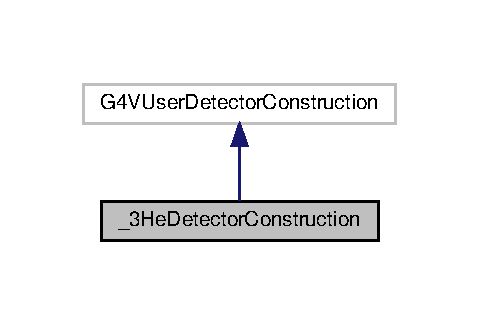
\includegraphics[width=230pt]{class__3HeDetectorConstruction__inherit__graph}
\end{center}
\end{figure}


Collaboration diagram for \+\_\+3\+He\+Detector\+Construction\+:
\nopagebreak
\begin{figure}[H]
\begin{center}
\leavevmode
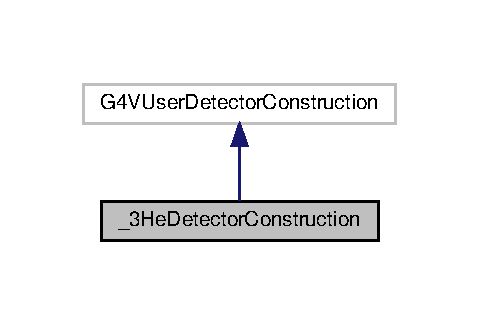
\includegraphics[width=230pt]{class__3HeDetectorConstruction__coll__graph}
\end{center}
\end{figure}
\subsection*{Public Member Functions}
\begin{DoxyCompactItemize}
\item 
\mbox{\Hypertarget{class__3HeDetectorConstruction_a77db6b8f95650831b38afa06616cbaef}\label{class__3HeDetectorConstruction_a77db6b8f95650831b38afa06616cbaef}} 
virtual G4\+V\+Physical\+Volume $\ast$ {\bfseries Construct} ()
\end{DoxyCompactItemize}


The documentation for this class was generated from the following files\+:\begin{DoxyCompactItemize}
\item 
include/\hyperlink{3HeDetectorConstruction_8hh}{3\+He\+Detector\+Construction.\+hh}\item 
src/\hyperlink{3HeDetectorConstruction_8cc}{3\+He\+Detector\+Construction.\+cc}\end{DoxyCompactItemize}

\hypertarget{class__3HeWorldConstruction}{}\section{\+\_\+3\+He\+World\+Construction Class Reference}
\label{class__3HeWorldConstruction}\index{\+\_\+3\+He\+World\+Construction@{\+\_\+3\+He\+World\+Construction}}


Inheritance diagram for \+\_\+3\+He\+World\+Construction\+:
\nopagebreak
\begin{figure}[H]
\begin{center}
\leavevmode
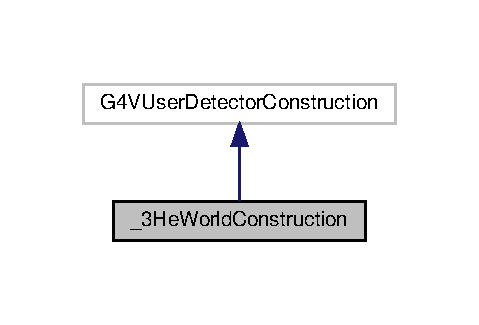
\includegraphics[width=230pt]{class__3HeWorldConstruction__inherit__graph}
\end{center}
\end{figure}


Collaboration diagram for \+\_\+3\+He\+World\+Construction\+:
\nopagebreak
\begin{figure}[H]
\begin{center}
\leavevmode
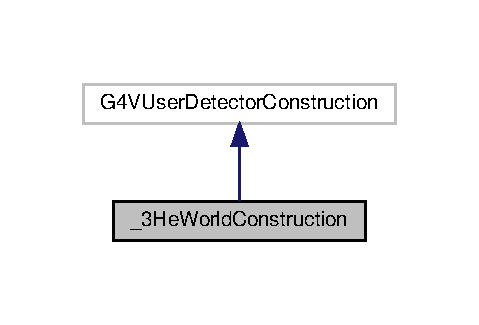
\includegraphics[width=230pt]{class__3HeWorldConstruction__coll__graph}
\end{center}
\end{figure}
\subsection*{Public Member Functions}
\begin{DoxyCompactItemize}
\item 
\mbox{\Hypertarget{class__3HeWorldConstruction_a123c069f0c962487d3dcb9e2f8dbc0b3}\label{class__3HeWorldConstruction_a123c069f0c962487d3dcb9e2f8dbc0b3}} 
virtual G4\+V\+Physical\+Volume $\ast$ {\bfseries Construct} ()
\end{DoxyCompactItemize}


The documentation for this class was generated from the following files\+:\begin{DoxyCompactItemize}
\item 
include/\hyperlink{3HeWorldConstruction_8hh}{3\+He\+World\+Construction.\+hh}\item 
src/\hyperlink{3HeWorldConstruction_8cc}{3\+He\+World\+Construction.\+cc}\end{DoxyCompactItemize}

\hypertarget{class__4HeDetectorConstruction}{}\section{\+\_\+4\+He\+Detector\+Construction Class Reference}
\label{class__4HeDetectorConstruction}\index{\+\_\+4\+He\+Detector\+Construction@{\+\_\+4\+He\+Detector\+Construction}}


Inheritance diagram for \+\_\+4\+He\+Detector\+Construction\+:
\nopagebreak
\begin{figure}[H]
\begin{center}
\leavevmode
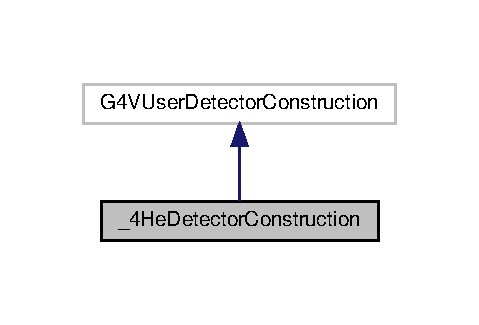
\includegraphics[width=230pt]{class__4HeDetectorConstruction__inherit__graph}
\end{center}
\end{figure}


Collaboration diagram for \+\_\+4\+He\+Detector\+Construction\+:
\nopagebreak
\begin{figure}[H]
\begin{center}
\leavevmode
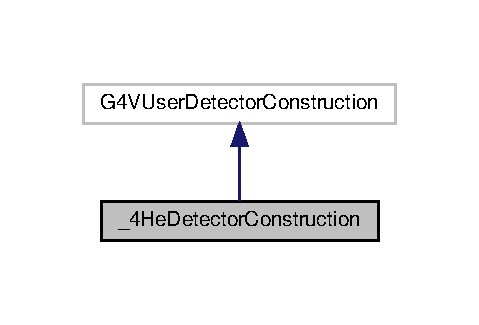
\includegraphics[width=230pt]{class__4HeDetectorConstruction__coll__graph}
\end{center}
\end{figure}
\subsection*{Public Member Functions}
\begin{DoxyCompactItemize}
\item 
\mbox{\Hypertarget{class__4HeDetectorConstruction_afaadb532467d010a0d024e5ea5fcbff2}\label{class__4HeDetectorConstruction_afaadb532467d010a0d024e5ea5fcbff2}} 
virtual G4\+V\+Physical\+Volume $\ast$ {\bfseries Construct} ()
\end{DoxyCompactItemize}


The documentation for this class was generated from the following files\+:\begin{DoxyCompactItemize}
\item 
include/\hyperlink{4HeDetectorConstruction_8hh}{4\+He\+Detector\+Construction.\+hh}\item 
src/\hyperlink{4HeDetectorConstruction_8cc}{4\+He\+Detector\+Construction.\+cc}\end{DoxyCompactItemize}

\hypertarget{classBF3DetectorConstruction}{}\section{B\+F3\+Detector\+Construction Class Reference}
\label{classBF3DetectorConstruction}\index{B\+F3\+Detector\+Construction@{B\+F3\+Detector\+Construction}}


Inheritance diagram for B\+F3\+Detector\+Construction\+:
\nopagebreak
\begin{figure}[H]
\begin{center}
\leavevmode
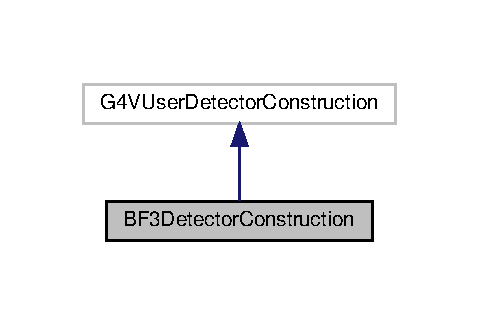
\includegraphics[width=230pt]{classBF3DetectorConstruction__inherit__graph}
\end{center}
\end{figure}


Collaboration diagram for B\+F3\+Detector\+Construction\+:
\nopagebreak
\begin{figure}[H]
\begin{center}
\leavevmode
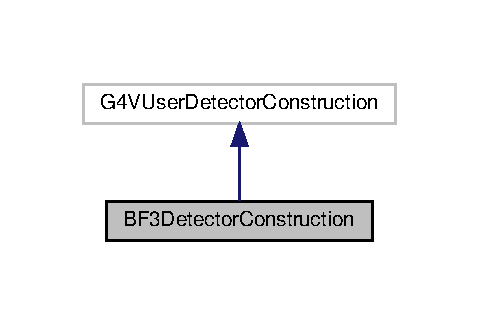
\includegraphics[width=230pt]{classBF3DetectorConstruction__coll__graph}
\end{center}
\end{figure}
\subsection*{Public Member Functions}
\begin{DoxyCompactItemize}
\item 
\mbox{\Hypertarget{classBF3DetectorConstruction_af683594ad695382e3e4e1ced109c71cb}\label{classBF3DetectorConstruction_af683594ad695382e3e4e1ced109c71cb}} 
virtual G4\+V\+Physical\+Volume $\ast$ {\bfseries Construct} ()
\end{DoxyCompactItemize}


The documentation for this class was generated from the following files\+:\begin{DoxyCompactItemize}
\item 
include/\hyperlink{BF3DetectorConstruction_8hh}{B\+F3\+Detector\+Construction.\+hh}\item 
src/\hyperlink{BF3DetectorConstruction_8cc}{B\+F3\+Detector\+Construction.\+cc}\end{DoxyCompactItemize}

\hypertarget{classCounterSD}{}\section{Counter\+SD Class Reference}
\label{classCounterSD}\index{Counter\+SD@{Counter\+SD}}


Inheritance diagram for Counter\+SD\+:
\nopagebreak
\begin{figure}[H]
\begin{center}
\leavevmode
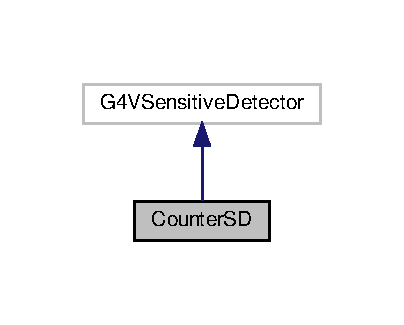
\includegraphics[width=194pt]{classCounterSD__inherit__graph}
\end{center}
\end{figure}


Collaboration diagram for Counter\+SD\+:
\nopagebreak
\begin{figure}[H]
\begin{center}
\leavevmode
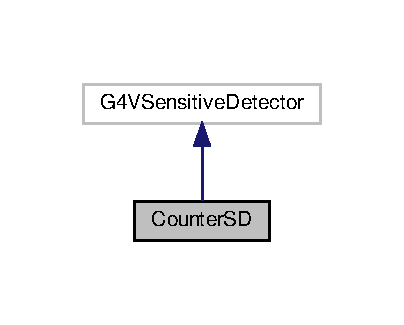
\includegraphics[width=194pt]{classCounterSD__coll__graph}
\end{center}
\end{figure}
\subsection*{Public Member Functions}
\begin{DoxyCompactItemize}
\item 
\mbox{\Hypertarget{classCounterSD_a47a5f480d0177da68a25ccde4ef26403}\label{classCounterSD_a47a5f480d0177da68a25ccde4ef26403}} 
{\bfseries Counter\+SD} (G4\+String id)
\item 
\mbox{\Hypertarget{classCounterSD_acca87f1f1f5235ed58d46f8e216a82ff}\label{classCounterSD_acca87f1f1f5235ed58d46f8e216a82ff}} 
virtual void {\bfseries Initialize} (G4\+H\+Cof\+This\+Event $\ast$H\+CE)
\item 
\mbox{\Hypertarget{classCounterSD_aeb540c654a6c5034d69835366d09ddb0}\label{classCounterSD_aeb540c654a6c5034d69835366d09ddb0}} 
virtual G4bool {\bfseries Process\+Hits} (G4\+Step $\ast$step, G4\+Touchable\+History $\ast$hist)
\end{DoxyCompactItemize}


The documentation for this class was generated from the following files\+:\begin{DoxyCompactItemize}
\item 
include/\hyperlink{CounterSD_8hh}{Counter\+S\+D.\+hh}\item 
src/\hyperlink{CounterSD_8cc}{Counter\+S\+D.\+cc}\end{DoxyCompactItemize}

\hypertarget{structGTKBoxesContainer}{}\section{G\+T\+K\+Boxes\+Container Struct Reference}
\label{structGTKBoxesContainer}\index{G\+T\+K\+Boxes\+Container@{G\+T\+K\+Boxes\+Container}}


Collaboration diagram for G\+T\+K\+Boxes\+Container\+:
\nopagebreak
\begin{figure}[H]
\begin{center}
\leavevmode
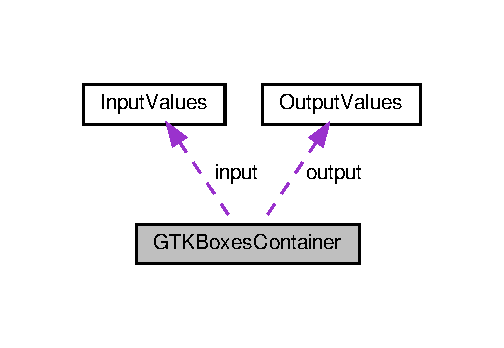
\includegraphics[width=242pt]{structGTKBoxesContainer__coll__graph}
\end{center}
\end{figure}
\subsection*{Public Attributes}
\begin{DoxyCompactItemize}
\item 
\mbox{\Hypertarget{structGTKBoxesContainer_acbdbbc58bb89072abb323d27d9ba4f9e}\label{structGTKBoxesContainer_acbdbbc58bb89072abb323d27d9ba4f9e}} 
Gtk\+Widget $\ast$ {\bfseries world\+\_\+material}
\item 
\mbox{\Hypertarget{structGTKBoxesContainer_aa5d9a558032880dc9c75da2310eed385}\label{structGTKBoxesContainer_aa5d9a558032880dc9c75da2310eed385}} 
Gtk\+Widget $\ast$ {\bfseries initial\+\_\+events}
\item 
\mbox{\Hypertarget{structGTKBoxesContainer_ae3293caaf4b63043ce80c225513e10e7}\label{structGTKBoxesContainer_ae3293caaf4b63043ce80c225513e10e7}} 
Gtk\+Widget $\ast$ {\bfseries neutron\+\_\+energy}
\item 
\mbox{\Hypertarget{structGTKBoxesContainer_a56dc6c28ec9242c0668cc2a14e33fc06}\label{structGTKBoxesContainer_a56dc6c28ec9242c0668cc2a14e33fc06}} 
Gtk\+Widget $\ast$ {\bfseries window}
\item 
\mbox{\Hypertarget{structGTKBoxesContainer_af90756c5ab7e0d1f9c9a5e1c328960cb}\label{structGTKBoxesContainer_af90756c5ab7e0d1f9c9a5e1c328960cb}} 
struct \hyperlink{classInputValues}{Input\+Values} $\ast$ {\bfseries input}
\item 
\mbox{\Hypertarget{structGTKBoxesContainer_aa60108d0377538098212c3b870b48bf3}\label{structGTKBoxesContainer_aa60108d0377538098212c3b870b48bf3}} 
struct \hyperlink{classOutputValues}{Output\+Values} $\ast$ {\bfseries output}
\end{DoxyCompactItemize}


The documentation for this struct was generated from the following file\+:\begin{DoxyCompactItemize}
\item 
include/\hyperlink{GTKInput_8hh}{G\+T\+K\+Input.\+hh}\end{DoxyCompactItemize}

\hypertarget{classHistogramsAnalysisManager}{}\section{Histograms\+Analysis\+Manager Class Reference}
\label{classHistogramsAnalysisManager}\index{Histograms\+Analysis\+Manager@{Histograms\+Analysis\+Manager}}


The documentation for this class was generated from the following files\+:\begin{DoxyCompactItemize}
\item 
include/\hyperlink{HistogramsAnalysisManager_8hh}{Histograms\+Analysis\+Manager.\+hh}\item 
src/\hyperlink{HistogramsAnalysisManager_8cc}{Histograms\+Analysis\+Manager.\+cc}\end{DoxyCompactItemize}

\hypertarget{classInputValues}{}\section{Input\+Values Class Reference}
\label{classInputValues}\index{Input\+Values@{Input\+Values}}
\subsection*{Public Attributes}
\begin{DoxyCompactItemize}
\item 
\mbox{\Hypertarget{classInputValues_a1054439a15815d3fe7161cae77bca497}\label{classInputValues_a1054439a15815d3fe7161cae77bca497}} 
std\+::string {\bfseries world\+\_\+material}
\item 
\mbox{\Hypertarget{classInputValues_a629e3a93c73d05dd50d5ec55845a0c35}\label{classInputValues_a629e3a93c73d05dd50d5ec55845a0c35}} 
int {\bfseries num\+\_\+events} = 100
\item 
\mbox{\Hypertarget{classInputValues_abc160a2cae57302dacc29ea8b3f748c6}\label{classInputValues_abc160a2cae57302dacc29ea8b3f748c6}} 
long double {\bfseries neutron\+\_\+energy} = 0.\+025
\item 
\mbox{\Hypertarget{classInputValues_afb1006c81c63900dce636b8252a8ea73}\label{classInputValues_afb1006c81c63900dce636b8252a8ea73}} 
enum Detector {\bfseries detector\+\_\+material}
\end{DoxyCompactItemize}


The documentation for this class was generated from the following file\+:\begin{DoxyCompactItemize}
\item 
include/\hyperlink{GTKInput_8hh}{G\+T\+K\+Input.\+hh}\end{DoxyCompactItemize}

\hypertarget{classMultipleWorldConstruction}{}\section{Multiple\+World\+Construction Class Reference}
\label{classMultipleWorldConstruction}\index{Multiple\+World\+Construction@{Multiple\+World\+Construction}}


Inheritance diagram for Multiple\+World\+Construction\+:
\nopagebreak
\begin{figure}[H]
\begin{center}
\leavevmode
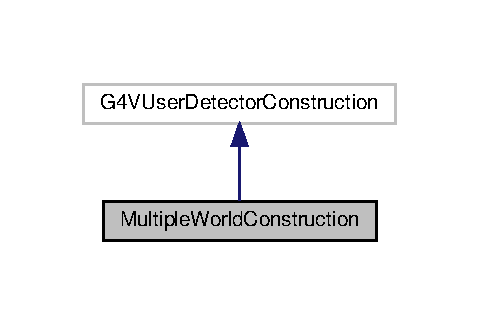
\includegraphics[width=230pt]{classMultipleWorldConstruction__inherit__graph}
\end{center}
\end{figure}


Collaboration diagram for Multiple\+World\+Construction\+:
\nopagebreak
\begin{figure}[H]
\begin{center}
\leavevmode
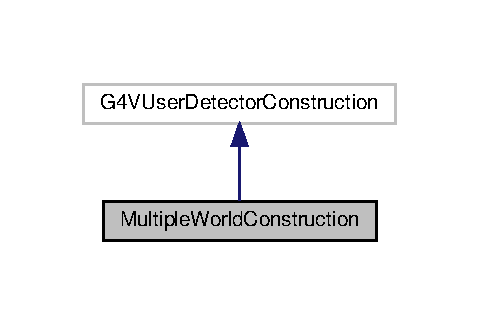
\includegraphics[width=230pt]{classMultipleWorldConstruction__coll__graph}
\end{center}
\end{figure}
\subsection*{Public Member Functions}
\begin{DoxyCompactItemize}
\item 
\mbox{\Hypertarget{classMultipleWorldConstruction_a9938de8bb542846fb6a19988baeb5de4}\label{classMultipleWorldConstruction_a9938de8bb542846fb6a19988baeb5de4}} 
virtual G4\+V\+Physical\+Volume $\ast$ \hyperlink{classMultipleWorldConstruction_a9938de8bb542846fb6a19988baeb5de4}{Construct} ()
\begin{DoxyCompactList}\small\item\em constructs the world, empty world with logical volume based on user-\/selected material \end{DoxyCompactList}\end{DoxyCompactItemize}


The documentation for this class was generated from the following files\+:\begin{DoxyCompactItemize}
\item 
include/\hyperlink{MultipleWorldConstruction_8hh}{Multiple\+World\+Construction.\+hh}\item 
src/\hyperlink{MultipleWorldConstruction_8cc}{Multiple\+World\+Construction.\+cc}\end{DoxyCompactItemize}

\hypertarget{classNeutronActionInitialization}{}\section{Neutron\+Action\+Initialization Class Reference}
\label{classNeutronActionInitialization}\index{Neutron\+Action\+Initialization@{Neutron\+Action\+Initialization}}


Inheritance diagram for Neutron\+Action\+Initialization\+:
\nopagebreak
\begin{figure}[H]
\begin{center}
\leavevmode
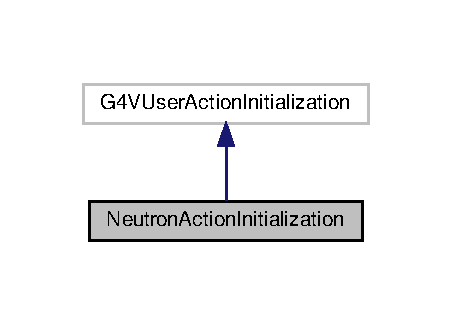
\includegraphics[width=217pt]{classNeutronActionInitialization__inherit__graph}
\end{center}
\end{figure}


Collaboration diagram for Neutron\+Action\+Initialization\+:
\nopagebreak
\begin{figure}[H]
\begin{center}
\leavevmode
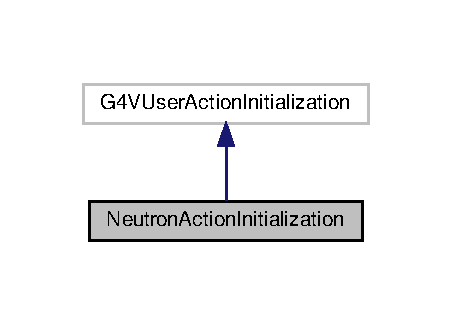
\includegraphics[width=217pt]{classNeutronActionInitialization__coll__graph}
\end{center}
\end{figure}
\subsection*{Public Member Functions}
\begin{DoxyCompactItemize}
\item 
\mbox{\Hypertarget{classNeutronActionInitialization_ab2f0627113890a43d8af4c2a45e96221}\label{classNeutronActionInitialization_ab2f0627113890a43d8af4c2a45e96221}} 
virtual void {\bfseries Build\+For\+Master} () const
\item 
\mbox{\Hypertarget{classNeutronActionInitialization_adc68464246541e3f72e3674bd235f658}\label{classNeutronActionInitialization_adc68464246541e3f72e3674bd235f658}} 
virtual void \hyperlink{classNeutronActionInitialization_adc68464246541e3f72e3674bd235f658}{Build} () const
\begin{DoxyCompactList}\small\item\em adds our user actions to a non-\/multithreaded run manager. \end{DoxyCompactList}\end{DoxyCompactItemize}


The documentation for this class was generated from the following files\+:\begin{DoxyCompactItemize}
\item 
include/\hyperlink{NeutronActionInitialization_8hh}{Neutron\+Action\+Initialization.\+hh}\item 
src/\hyperlink{NeutronActionInitialization_8cc}{Neutron\+Action\+Initialization.\+cc}\end{DoxyCompactItemize}

\hypertarget{classNeutronPrimaryGeneratorAction}{}\section{Neutron\+Primary\+Generator\+Action Class Reference}
\label{classNeutronPrimaryGeneratorAction}\index{Neutron\+Primary\+Generator\+Action@{Neutron\+Primary\+Generator\+Action}}


Inheritance diagram for Neutron\+Primary\+Generator\+Action\+:
\nopagebreak
\begin{figure}[H]
\begin{center}
\leavevmode
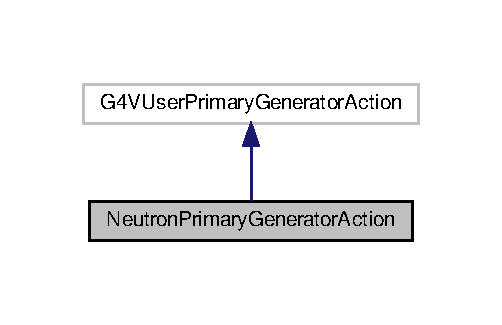
\includegraphics[width=241pt]{classNeutronPrimaryGeneratorAction__inherit__graph}
\end{center}
\end{figure}


Collaboration diagram for Neutron\+Primary\+Generator\+Action\+:
\nopagebreak
\begin{figure}[H]
\begin{center}
\leavevmode
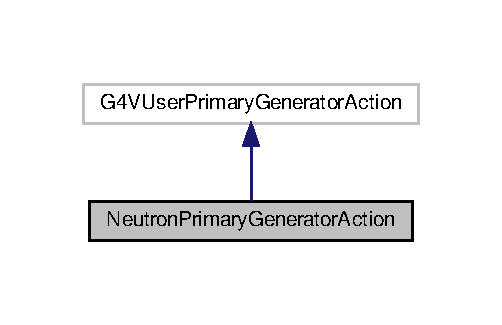
\includegraphics[width=241pt]{classNeutronPrimaryGeneratorAction__coll__graph}
\end{center}
\end{figure}
\subsection*{Public Member Functions}
\begin{DoxyCompactItemize}
\item 
\mbox{\Hypertarget{classNeutronPrimaryGeneratorAction_a58464b853d6e69d3a631dd1ce70e68aa}\label{classNeutronPrimaryGeneratorAction_a58464b853d6e69d3a631dd1ce70e68aa}} 
\hyperlink{classNeutronPrimaryGeneratorAction_a58464b853d6e69d3a631dd1ce70e68aa}{Neutron\+Primary\+Generator\+Action} ()
\begin{DoxyCompactList}\small\item\em computes the desired primary particle properties, initializes the neutron gun so that the Event class can access it. \end{DoxyCompactList}\item 
\mbox{\Hypertarget{classNeutronPrimaryGeneratorAction_afa37cc6fbe070f397780f5da1b4b015d}\label{classNeutronPrimaryGeneratorAction_afa37cc6fbe070f397780f5da1b4b015d}} 
virtual void \hyperlink{classNeutronPrimaryGeneratorAction_afa37cc6fbe070f397780f5da1b4b015d}{Generate\+Primaries} (G4\+Event $\ast$)
\begin{DoxyCompactList}\small\item\em called for the number of times we specify using /run/\+Beam\+On \end{DoxyCompactList}\item 
\mbox{\Hypertarget{classNeutronPrimaryGeneratorAction_a34bc9633aaaf6d123a9bd59fb736732b}\label{classNeutronPrimaryGeneratorAction_a34bc9633aaaf6d123a9bd59fb736732b}} 
G4\+Particle\+Gun $\ast$ \hyperlink{classNeutronPrimaryGeneratorAction_a34bc9633aaaf6d123a9bd59fb736732b}{Get\+Particle\+Gun} ()
\begin{DoxyCompactList}\small\item\em used by the \hyperlink{classNeutronRunAction}{Neutron\+Run\+Action} class to get the particle gun \end{DoxyCompactList}\end{DoxyCompactItemize}


The documentation for this class was generated from the following files\+:\begin{DoxyCompactItemize}
\item 
include/\hyperlink{NeutronPrimaryGeneratorAction_8hh}{Neutron\+Primary\+Generator\+Action.\+hh}\item 
src/\hyperlink{NeutronPrimaryGeneratorAction_8cc}{Neutron\+Primary\+Generator\+Action.\+cc}\end{DoxyCompactItemize}

\hypertarget{classNeutronRunAction}{}\section{Neutron\+Run\+Action Class Reference}
\label{classNeutronRunAction}\index{Neutron\+Run\+Action@{Neutron\+Run\+Action}}


Inheritance diagram for Neutron\+Run\+Action\+:
\nopagebreak
\begin{figure}[H]
\begin{center}
\leavevmode
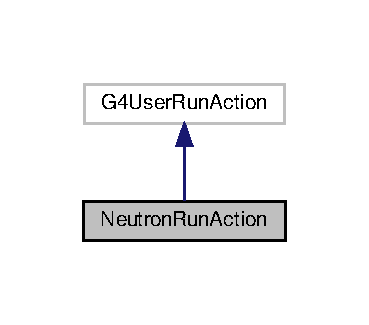
\includegraphics[width=177pt]{classNeutronRunAction__inherit__graph}
\end{center}
\end{figure}


Collaboration diagram for Neutron\+Run\+Action\+:
\nopagebreak
\begin{figure}[H]
\begin{center}
\leavevmode
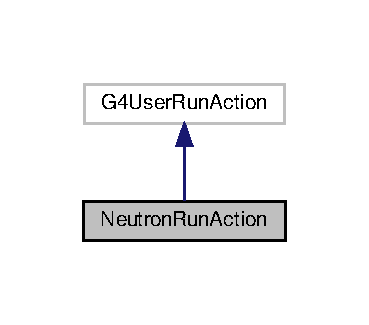
\includegraphics[width=177pt]{classNeutronRunAction__coll__graph}
\end{center}
\end{figure}
\subsection*{Public Member Functions}
\begin{DoxyCompactItemize}
\item 
\mbox{\Hypertarget{classNeutronRunAction_aedf76bb3ee1a8fb0bf0d626ec8939465}\label{classNeutronRunAction_aedf76bb3ee1a8fb0bf0d626ec8939465}} 
{\bfseries Neutron\+Run\+Action} (\hyperlink{classNeutronPrimaryGeneratorAction}{Neutron\+Primary\+Generator\+Action} $\ast$particle\+\_\+gun\+\_\+info)
\item 
\mbox{\Hypertarget{classNeutronRunAction_a9dce5b57c14691296f1705f57074d8af}\label{classNeutronRunAction_a9dce5b57c14691296f1705f57074d8af}} 
virtual G4\+Run $\ast$ {\bfseries Generate\+Run} ()
\item 
\mbox{\Hypertarget{classNeutronRunAction_afe9e7f70040e7ca3bed78ac2234726d1}\label{classNeutronRunAction_afe9e7f70040e7ca3bed78ac2234726d1}} 
virtual void {\bfseries Begin\+Of\+Run\+Action} (const G4\+Run $\ast$run)
\item 
\mbox{\Hypertarget{classNeutronRunAction_afaa663339bbeaf39a71b5e3052be367e}\label{classNeutronRunAction_afaa663339bbeaf39a71b5e3052be367e}} 
virtual void {\bfseries End\+Of\+Run\+Action} (const G4\+Run $\ast$run)
\end{DoxyCompactItemize}


The documentation for this class was generated from the following files\+:\begin{DoxyCompactItemize}
\item 
include/\hyperlink{NeutronRunAction_8hh}{Neutron\+Run\+Action.\+hh}\item 
src/\hyperlink{NeutronRunAction_8cc}{Neutron\+Run\+Action.\+cc}\end{DoxyCompactItemize}

\hypertarget{classOutputValues}{}\section{Output\+Values Class Reference}
\label{classOutputValues}\index{Output\+Values@{Output\+Values}}
\subsection*{Public Attributes}
\begin{DoxyCompactItemize}
\item 
\mbox{\Hypertarget{classOutputValues_a013df34f07ece3c720cfa3ef462baf82}\label{classOutputValues_a013df34f07ece3c720cfa3ef462baf82}} 
long double {\bfseries edep\+\_\+target}
\item 
\mbox{\Hypertarget{classOutputValues_a8db6b22c65174226bf75b264c429139d}\label{classOutputValues_a8db6b22c65174226bf75b264c429139d}} 
long double {\bfseries edep\+\_\+world} = 0.\+0
\item 
\mbox{\Hypertarget{classOutputValues_a85926d9c2fbd8967bd4bedc3cdc9a9ea}\label{classOutputValues_a85926d9c2fbd8967bd4bedc3cdc9a9ea}} 
long long {\bfseries nparticle\+\_\+target} = 0
\item 
\mbox{\Hypertarget{classOutputValues_a0ee5c2f5f8855873bf9a471eb795c297}\label{classOutputValues_a0ee5c2f5f8855873bf9a471eb795c297}} 
long long {\bfseries nneutron\+\_\+target} = 0
\item 
\mbox{\Hypertarget{classOutputValues_a4c57cdc9121114148179b250be9a3f55}\label{classOutputValues_a4c57cdc9121114148179b250be9a3f55}} 
std\+::string {\bfseries world\+\_\+material}
\item 
\mbox{\Hypertarget{classOutputValues_a7703523c094eb54aed884735f8811b5c}\label{classOutputValues_a7703523c094eb54aed884735f8811b5c}} 
std\+::string {\bfseries target\+\_\+material}
\item 
\mbox{\Hypertarget{classOutputValues_a00d3af733855600703105f6e9b423c52}\label{classOutputValues_a00d3af733855600703105f6e9b423c52}} 
long long {\bfseries nevent\+\_\+initial} = 0
\item 
\mbox{\Hypertarget{classOutputValues_adc64463195db40f08ccd9d64b9ff70b5}\label{classOutputValues_adc64463195db40f08ccd9d64b9ff70b5}} 
long double {\bfseries eneutron\+\_\+initial} = 0
\end{DoxyCompactItemize}


The documentation for this class was generated from the following file\+:\begin{DoxyCompactItemize}
\item 
include/\hyperlink{GTKInput_8hh}{G\+T\+K\+Input.\+hh}\end{DoxyCompactItemize}

\hypertarget{structWinContainer}{}\section{Win\+Container Struct Reference}
\label{structWinContainer}\index{Win\+Container@{Win\+Container}}
\subsection*{Public Attributes}
\begin{DoxyCompactItemize}
\item 
\mbox{\Hypertarget{structWinContainer_a6e871dba074f9e341c0341c7a5f91969}\label{structWinContainer_a6e871dba074f9e341c0341c7a5f91969}} 
Gtk\+Widget $\ast$ {\bfseries window}
\end{DoxyCompactItemize}


The documentation for this struct was generated from the following file\+:\begin{DoxyCompactItemize}
\item 
include/\hyperlink{GTKOutput_8hh}{G\+T\+K\+Output.\+hh}\end{DoxyCompactItemize}

\chapter{File Documentation}
\hypertarget{3HeDetectorConstruction_8hh}{}\section{include/3\+He\+Detector\+Construction.hh File Reference}
\label{3HeDetectorConstruction_8hh}\index{include/3\+He\+Detector\+Construction.\+hh@{include/3\+He\+Detector\+Construction.\+hh}}


header for the helium-\/3 detector construction  


{\ttfamily \#include \char`\"{}G4\+V\+User\+Detector\+Construction.\+hh\char`\"{}}\newline
Include dependency graph for 3\+He\+Detector\+Construction.hh\+:
\nopagebreak
\begin{figure}[H]
\begin{center}
\leavevmode
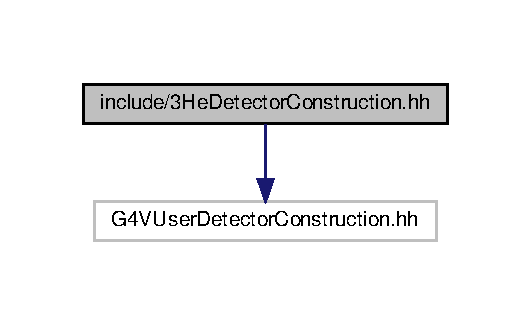
\includegraphics[width=255pt]{3HeDetectorConstruction_8hh__incl}
\end{center}
\end{figure}
This graph shows which files directly or indirectly include this file\+:
\nopagebreak
\begin{figure}[H]
\begin{center}
\leavevmode
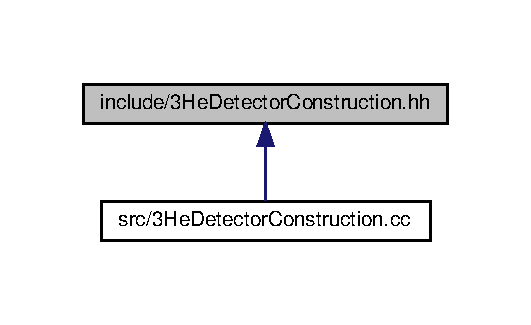
\includegraphics[width=255pt]{3HeDetectorConstruction_8hh__dep__incl}
\end{center}
\end{figure}
\subsection*{Classes}
\begin{DoxyCompactItemize}
\item 
class \hyperlink{class__3HeDetectorConstruction}{\+\_\+3\+He\+Detector\+Construction}
\end{DoxyCompactItemize}


\subsection{Detailed Description}
header for the helium-\/3 detector construction 

\begin{DoxyAuthor}{Author}
Oisin O\textquotesingle{}Connell 
\end{DoxyAuthor}
\begin{DoxyDate}{Date}
7/28/2020 
\end{DoxyDate}

\hypertarget{3HeWorldConstruction_8hh}{}\section{include/3\+He\+World\+Construction.hh File Reference}
\label{3HeWorldConstruction_8hh}\index{include/3\+He\+World\+Construction.\+hh@{include/3\+He\+World\+Construction.\+hh}}


helium-\/3 world envelope construction file.  


{\ttfamily \#include \char`\"{}G4\+V\+User\+Detector\+Construction.\+hh\char`\"{}}\newline
Include dependency graph for 3\+He\+World\+Construction.hh\+:
\nopagebreak
\begin{figure}[H]
\begin{center}
\leavevmode
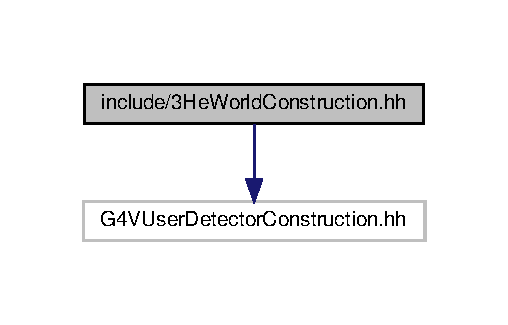
\includegraphics[width=244pt]{3HeWorldConstruction_8hh__incl}
\end{center}
\end{figure}
This graph shows which files directly or indirectly include this file\+:
\nopagebreak
\begin{figure}[H]
\begin{center}
\leavevmode
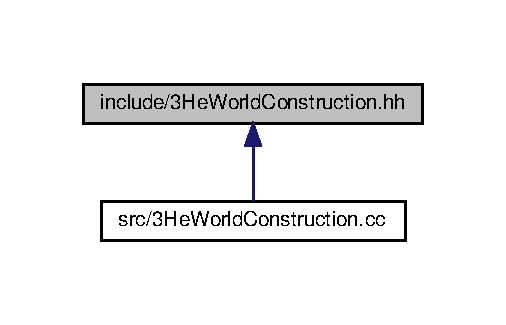
\includegraphics[width=243pt]{3HeWorldConstruction_8hh__dep__incl}
\end{center}
\end{figure}
\subsection*{Classes}
\begin{DoxyCompactItemize}
\item 
class \hyperlink{class__3HeWorldConstruction}{\+\_\+3\+He\+World\+Construction}
\end{DoxyCompactItemize}


\subsection{Detailed Description}
helium-\/3 world envelope construction file. 

\begin{DoxyAuthor}{Author}
Oisin O\textquotesingle{}Connell 
\end{DoxyAuthor}
\begin{DoxyDate}{Date}
7/28/2020 
\end{DoxyDate}

\hypertarget{4HeDetectorConstruction_8hh}{}\section{include/4\+He\+Detector\+Construction.hh File Reference}
\label{4HeDetectorConstruction_8hh}\index{include/4\+He\+Detector\+Construction.\+hh@{include/4\+He\+Detector\+Construction.\+hh}}


helium-\/4 container in an air world envelope detector construction header file  


{\ttfamily \#include \char`\"{}G4\+V\+User\+Detector\+Construction.\+hh\char`\"{}}\newline
Include dependency graph for 4\+He\+Detector\+Construction.hh\+:
\nopagebreak
\begin{figure}[H]
\begin{center}
\leavevmode
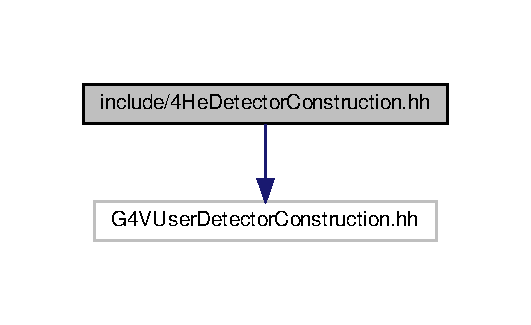
\includegraphics[width=255pt]{4HeDetectorConstruction_8hh__incl}
\end{center}
\end{figure}
This graph shows which files directly or indirectly include this file\+:
\nopagebreak
\begin{figure}[H]
\begin{center}
\leavevmode
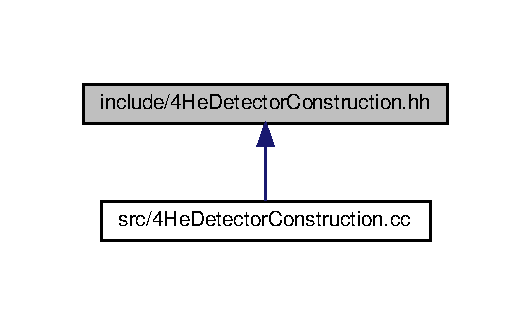
\includegraphics[width=255pt]{4HeDetectorConstruction_8hh__dep__incl}
\end{center}
\end{figure}
\subsection*{Classes}
\begin{DoxyCompactItemize}
\item 
class \hyperlink{class__4HeDetectorConstruction}{\+\_\+4\+He\+Detector\+Construction}
\end{DoxyCompactItemize}


\subsection{Detailed Description}
helium-\/4 container in an air world envelope detector construction header file 

\begin{DoxyAuthor}{Author}
Oisin O\textquotesingle{}Connell 
\end{DoxyAuthor}
\begin{DoxyDate}{Date}
7/28/2020 
\end{DoxyDate}

\hypertarget{BF3DetectorConstruction_8hh}{}\section{include/\+B\+F3\+Detector\+Construction.hh File Reference}
\label{BF3DetectorConstruction_8hh}\index{include/\+B\+F3\+Detector\+Construction.\+hh@{include/\+B\+F3\+Detector\+Construction.\+hh}}


boron trifluoride container in a modifiable world envelope detector construction header file  


{\ttfamily \#include \char`\"{}G4\+V\+User\+Detector\+Construction.\+hh\char`\"{}}\newline
Include dependency graph for B\+F3\+Detector\+Construction.\+hh\+:
\nopagebreak
\begin{figure}[H]
\begin{center}
\leavevmode
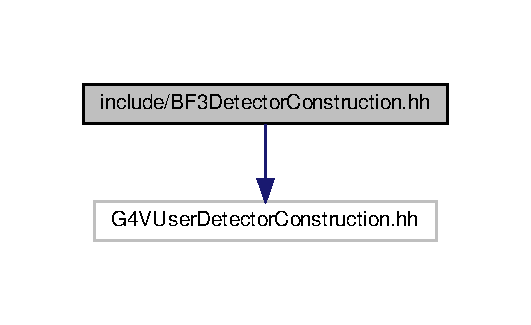
\includegraphics[width=255pt]{BF3DetectorConstruction_8hh__incl}
\end{center}
\end{figure}
This graph shows which files directly or indirectly include this file\+:
\nopagebreak
\begin{figure}[H]
\begin{center}
\leavevmode
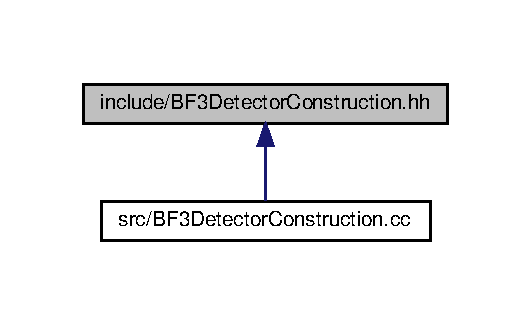
\includegraphics[width=255pt]{BF3DetectorConstruction_8hh__dep__incl}
\end{center}
\end{figure}
\subsection*{Classes}
\begin{DoxyCompactItemize}
\item 
class \hyperlink{classBF3DetectorConstruction}{B\+F3\+Detector\+Construction}
\end{DoxyCompactItemize}


\subsection{Detailed Description}
boron trifluoride container in a modifiable world envelope detector construction header file 

\begin{DoxyAuthor}{Author}
Oisin O\textquotesingle{}Connell 
\end{DoxyAuthor}
\begin{DoxyDate}{Date}
7/28/2020 
\end{DoxyDate}

\hypertarget{CounterSD_8hh}{}\section{include/\+Counter\+SD.hh File Reference}
\label{CounterSD_8hh}\index{include/\+Counter\+S\+D.\+hh@{include/\+Counter\+S\+D.\+hh}}


sensitive detector definition header file.  


{\ttfamily \#include \char`\"{}G4\+V\+Sensitive\+Detector.\+hh\char`\"{}}\newline
{\ttfamily \#include \char`\"{}G4\+Particle\+Types.\+hh\char`\"{}}\newline
{\ttfamily \#include \char`\"{}g4csv.\+hh\char`\"{}}\newline
Include dependency graph for Counter\+S\+D.\+hh\+:
\nopagebreak
\begin{figure}[H]
\begin{center}
\leavevmode
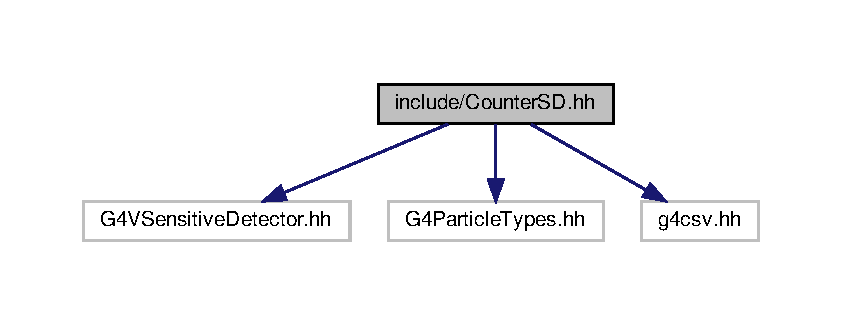
\includegraphics[width=350pt]{CounterSD_8hh__incl}
\end{center}
\end{figure}
This graph shows which files directly or indirectly include this file\+:
\nopagebreak
\begin{figure}[H]
\begin{center}
\leavevmode
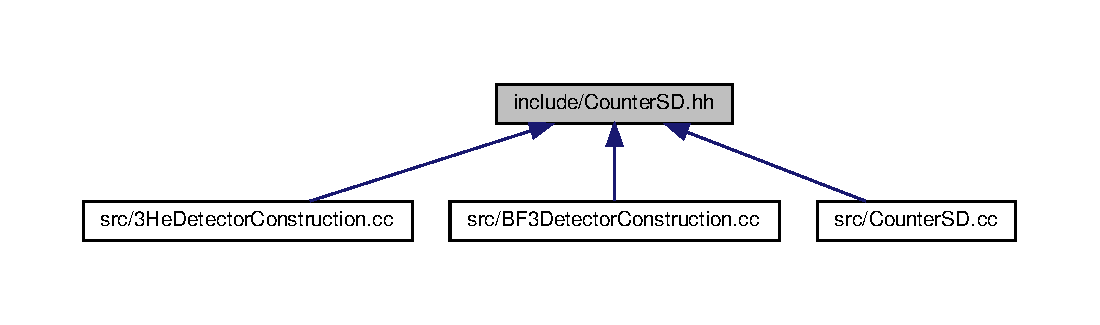
\includegraphics[width=350pt]{CounterSD_8hh__dep__incl}
\end{center}
\end{figure}
\subsection*{Classes}
\begin{DoxyCompactItemize}
\item 
class \hyperlink{classCounterSD}{Counter\+SD}
\end{DoxyCompactItemize}


\subsection{Detailed Description}
sensitive detector definition header file. 

\begin{DoxyAuthor}{Author}
Oisin O\textquotesingle{}Connell 
\end{DoxyAuthor}
\begin{DoxyDate}{Date}
7/28/2020 
\end{DoxyDate}

\hypertarget{global__materials_8hh}{}\section{include/global\+\_\+materials.hh File Reference}
\label{global__materials_8hh}\index{include/global\+\_\+materials.\+hh@{include/global\+\_\+materials.\+hh}}


global materials file, if the get\+\_\+input() function is used to get the propagation material in main, this file contains the results which we can use to select the material.  


\subsection*{Variables}
\begin{DoxyCompactItemize}
\item 
\mbox{\Hypertarget{global__materials_8hh_a93d9d1add1c17e2ae9723c89f77f047f}\label{global__materials_8hh_a93d9d1add1c17e2ae9723c89f77f047f}} 
int {\bfseries S\+P\+A\+C\+E\+\_\+\+S\+E\+L\+E\+C\+T\+ED}
\item 
\mbox{\Hypertarget{global__materials_8hh_af1d2cdb32af85fa8dcc407090d968c52}\label{global__materials_8hh_af1d2cdb32af85fa8dcc407090d968c52}} 
int {\bfseries W\+A\+T\+E\+R\+\_\+\+S\+E\+L\+E\+C\+T\+ED}
\item 
\mbox{\Hypertarget{global__materials_8hh_a2949513d4205c97accdb512267b16078}\label{global__materials_8hh_a2949513d4205c97accdb512267b16078}} 
int {\bfseries A\+I\+R\+\_\+\+S\+E\+L\+E\+C\+T\+ED}
\item 
\mbox{\Hypertarget{global__materials_8hh_a74dc696d6118c25b84a895708dacf92a}\label{global__materials_8hh_a74dc696d6118c25b84a895708dacf92a}} 
int {\bfseries A\+R\+G\+O\+N\+\_\+\+S\+E\+L\+E\+C\+T\+ED}
\item 
\mbox{\Hypertarget{global__materials_8hh_a5791b97ab4cdc578a6e9f013484d87ac}\label{global__materials_8hh_a5791b97ab4cdc578a6e9f013484d87ac}} 
int {\bfseries H\+E\+L\+I\+U\+M\+\_\+\+S\+E\+L\+E\+C\+T\+ED}
\end{DoxyCompactItemize}


\subsection{Detailed Description}
global materials file, if the get\+\_\+input() function is used to get the propagation material in main, this file contains the results which we can use to select the material. 

\begin{DoxyAuthor}{Author}
Oisin O\textquotesingle{}Connell 
\end{DoxyAuthor}
\begin{DoxyDate}{Date}
7/29/2020 
\end{DoxyDate}

\hypertarget{GTKInput_8hh}{}\section{include/\+G\+T\+K\+Input.hh File Reference}
\label{GTKInput_8hh}\index{include/\+G\+T\+K\+Input.\+hh@{include/\+G\+T\+K\+Input.\+hh}}


G\+TK input header file, allows user to input the material for the neutrons to propagate through and collects the user input in a struct that is used by the detector construction and the primary generator action to create a customized simulation.  


{\ttfamily \#include $<$gtk/gtk.\+h$>$}\newline
{\ttfamily \#include $<$iostream$>$}\newline
{\ttfamily \#include $<$vector$>$}\newline
Include dependency graph for G\+T\+K\+Input.\+hh\+:
\nopagebreak
\begin{figure}[H]
\begin{center}
\leavevmode
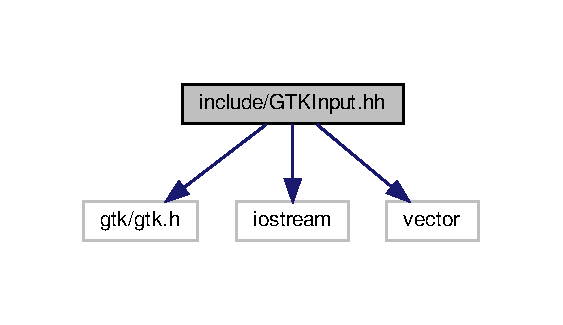
\includegraphics[width=270pt]{GTKInput_8hh__incl}
\end{center}
\end{figure}
This graph shows which files directly or indirectly include this file\+:
\nopagebreak
\begin{figure}[H]
\begin{center}
\leavevmode
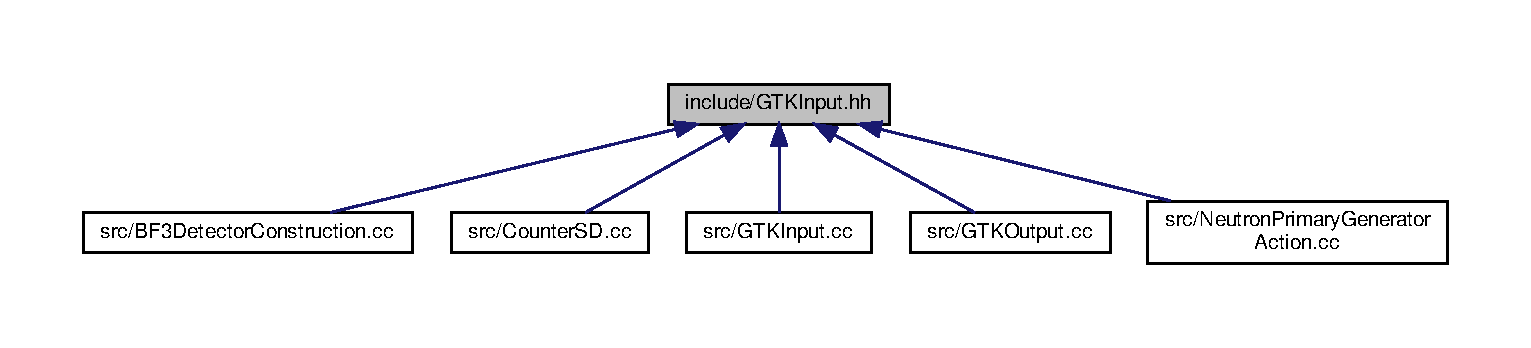
\includegraphics[width=350pt]{GTKInput_8hh__dep__incl}
\end{center}
\end{figure}
\subsection*{Classes}
\begin{DoxyCompactItemize}
\item 
class \hyperlink{classInputValues}{Input\+Values}
\item 
class \hyperlink{classOutputValues}{Output\+Values}
\item 
struct \hyperlink{structGTKBoxesContainer}{G\+T\+K\+Boxes\+Container}
\end{DoxyCompactItemize}
\subsection*{Enumerations}
\begin{DoxyCompactItemize}
\item 
\mbox{\Hypertarget{GTKInput_8hh_a2331baf03bacdf22d5763e6ce3329e2f}\label{GTKInput_8hh_a2331baf03bacdf22d5763e6ce3329e2f}} 
enum {\bfseries Detector} 
\end{DoxyCompactItemize}
\subsection*{Functions}
\begin{DoxyCompactItemize}
\item 
\mbox{\Hypertarget{GTKInput_8hh_a19f5912b30e5d38df0a3c0bfa9b794f2}\label{GTKInput_8hh_a19f5912b30e5d38df0a3c0bfa9b794f2}} 
void {\bfseries create\+\_\+data\+\_\+entry\+\_\+window} ()
\end{DoxyCompactItemize}
\subsection*{Variables}
\begin{DoxyCompactItemize}
\item 
\mbox{\Hypertarget{GTKInput_8hh_aefb2ae95fdd6ed4de4ff76a886180f24}\label{GTKInput_8hh_aefb2ae95fdd6ed4de4ff76a886180f24}} 
std\+::vector$<$ std\+::string $>$ {\bfseries detector\+\_\+materials}
\item 
\mbox{\Hypertarget{GTKInput_8hh_a69055fa214854d483b97260a00cbfa60}\label{GTKInput_8hh_a69055fa214854d483b97260a00cbfa60}} 
\hyperlink{classInputValues}{Input\+Values} $\ast$ {\bfseries input\+\_\+values}
\item 
\mbox{\Hypertarget{GTKInput_8hh_af802813aa13c8a2d9a86f12dc49d5c92}\label{GTKInput_8hh_af802813aa13c8a2d9a86f12dc49d5c92}} 
\hyperlink{classOutputValues}{Output\+Values} $\ast$ {\bfseries output\+\_\+values}
\item 
\mbox{\Hypertarget{GTKInput_8hh_a9af02616a624ef7c34dee19b71e0bf32}\label{GTKInput_8hh_a9af02616a624ef7c34dee19b71e0bf32}} 
struct \hyperlink{structGTKBoxesContainer}{G\+T\+K\+Boxes\+Container} $\ast$ {\bfseries results}
\end{DoxyCompactItemize}


\subsection{Detailed Description}
G\+TK input header file, allows user to input the material for the neutrons to propagate through and collects the user input in a struct that is used by the detector construction and the primary generator action to create a customized simulation. 

\begin{DoxyAuthor}{Author}
Oisin O\textquotesingle{}Connell 
\end{DoxyAuthor}
\begin{DoxyDate}{Date}
7/29/2020 
\end{DoxyDate}

\hypertarget{GTKOutput_8hh}{}\section{include/\+G\+T\+K\+Output.hh File Reference}
\label{GTKOutput_8hh}\index{include/\+G\+T\+K\+Output.\+hh@{include/\+G\+T\+K\+Output.\+hh}}


G\+TK output header file, collects the results from the \hyperlink{classOutputValues}{Output\+Values} struct that is forward declared in the G\+T\+K\+Input header file and displays them as the output.  


{\ttfamily \#include $<$gtk/gtk.\+h$>$}\newline
{\ttfamily \#include $<$iostream$>$}\newline
Include dependency graph for G\+T\+K\+Output.\+hh\+:
\nopagebreak
\begin{figure}[H]
\begin{center}
\leavevmode
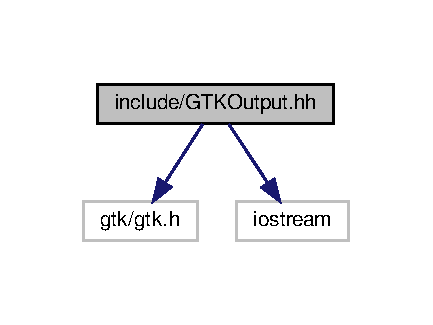
\includegraphics[width=208pt]{GTKOutput_8hh__incl}
\end{center}
\end{figure}
This graph shows which files directly or indirectly include this file\+:
\nopagebreak
\begin{figure}[H]
\begin{center}
\leavevmode
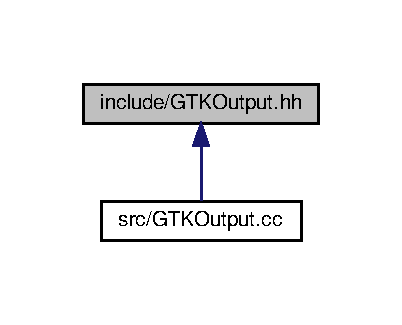
\includegraphics[width=193pt]{GTKOutput_8hh__dep__incl}
\end{center}
\end{figure}
\subsection*{Classes}
\begin{DoxyCompactItemize}
\item 
struct \hyperlink{structWinContainer}{Win\+Container}
\end{DoxyCompactItemize}
\subsection*{Functions}
\begin{DoxyCompactItemize}
\item 
void \hyperlink{GTKOutput_8hh_acc11cbf62638ba1237401d4346d86a1c}{close\+\_\+clicked} (Gtk\+Widget $\ast$button, struct \hyperlink{structWinContainer}{Win\+Container} $\ast$wc)
\begin{DoxyCompactList}\small\item\em callback that closes the window when the close button is clicked \end{DoxyCompactList}\item 
\mbox{\Hypertarget{GTKOutput_8hh_a6391991aa8e57c5bdfae21fb4fd8f707}\label{GTKOutput_8hh_a6391991aa8e57c5bdfae21fb4fd8f707}} 
void \hyperlink{GTKOutput_8hh_a6391991aa8e57c5bdfae21fb4fd8f707}{create\+\_\+output\+\_\+window} ()
\begin{DoxyCompactList}\small\item\em creates the output window that contains the energy deposition and other statistics after a simulation has run. \end{DoxyCompactList}\end{DoxyCompactItemize}


\subsection{Detailed Description}
G\+TK output header file, collects the results from the \hyperlink{classOutputValues}{Output\+Values} struct that is forward declared in the G\+T\+K\+Input header file and displays them as the output. 

\begin{DoxyAuthor}{Author}
Oisin O\textquotesingle{}Connell 
\end{DoxyAuthor}
\begin{DoxyDate}{Date}
7/29/2020 
\end{DoxyDate}


\subsection{Function Documentation}
\mbox{\Hypertarget{GTKOutput_8hh_acc11cbf62638ba1237401d4346d86a1c}\label{GTKOutput_8hh_acc11cbf62638ba1237401d4346d86a1c}} 
\index{G\+T\+K\+Output.\+hh@{G\+T\+K\+Output.\+hh}!close\+\_\+clicked@{close\+\_\+clicked}}
\index{close\+\_\+clicked@{close\+\_\+clicked}!G\+T\+K\+Output.\+hh@{G\+T\+K\+Output.\+hh}}
\subsubsection{\texorpdfstring{close\+\_\+clicked()}{close\_clicked()}}
{\footnotesize\ttfamily void close\+\_\+clicked (\begin{DoxyParamCaption}\item[{Gtk\+Widget $\ast$}]{button,  }\item[{struct \hyperlink{structWinContainer}{Win\+Container} $\ast$}]{wc }\end{DoxyParamCaption})}



callback that closes the window when the close button is clicked 


\begin{DoxyParams}{Parameters}
{\em button} & the button widget \\
\hline
{\em wc} & a struct containing the window that displays the results \\
\hline
\end{DoxyParams}

\hypertarget{HistogramsAnalysisManager_8hh}{}\section{include/\+Histograms\+Analysis\+Manager.hh File Reference}
\label{HistogramsAnalysisManager_8hh}\index{include/\+Histograms\+Analysis\+Manager.\+hh@{include/\+Histograms\+Analysis\+Manager.\+hh}}


Analysis manager header file, optionally allows us to place commands within our code that add to a histogram based on an event, a step, or something else.  


{\ttfamily \#include \char`\"{}g4csv.\+hh\char`\"{}}\newline
Include dependency graph for Histograms\+Analysis\+Manager.\+hh\+:
\nopagebreak
\begin{figure}[H]
\begin{center}
\leavevmode
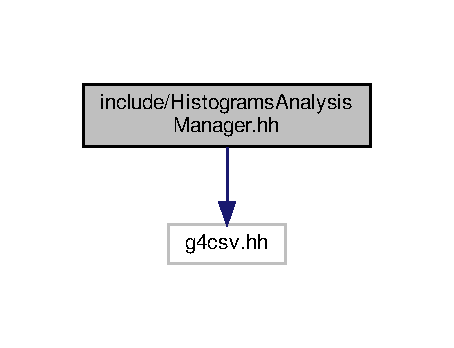
\includegraphics[width=218pt]{HistogramsAnalysisManager_8hh__incl}
\end{center}
\end{figure}
This graph shows which files directly or indirectly include this file\+:
\nopagebreak
\begin{figure}[H]
\begin{center}
\leavevmode
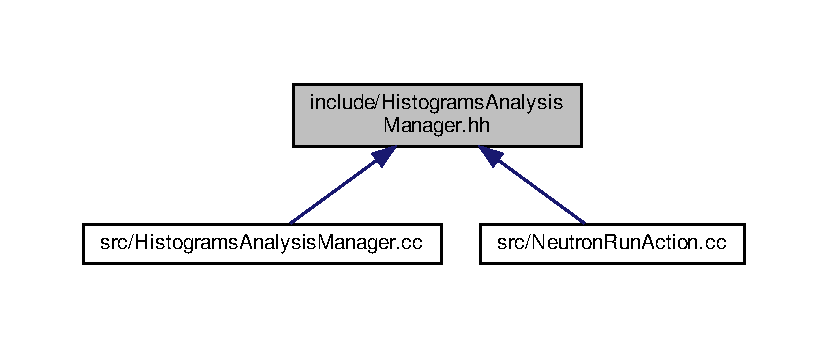
\includegraphics[width=350pt]{HistogramsAnalysisManager_8hh__dep__incl}
\end{center}
\end{figure}
\subsection*{Classes}
\begin{DoxyCompactItemize}
\item 
class \hyperlink{classHistogramsAnalysisManager}{Histograms\+Analysis\+Manager}
\end{DoxyCompactItemize}


\subsection{Detailed Description}
Analysis manager header file, optionally allows us to place commands within our code that add to a histogram based on an event, a step, or something else. 

\begin{DoxyAuthor}{Author}
Oisin O\textquotesingle{}Connell 
\end{DoxyAuthor}
\begin{DoxyDate}{Date}
7/29/2020 
\end{DoxyDate}

\hypertarget{MultipleWorldConstruction_8hh}{}\section{include/\+Multiple\+World\+Construction.hh File Reference}
\label{MultipleWorldConstruction_8hh}\index{include/\+Multiple\+World\+Construction.\+hh@{include/\+Multiple\+World\+Construction.\+hh}}


multiple world construction header file, when used allows us to choose the world based on the input that we receive from the get\+Input function in main, but by default we use a G\+TK window instead.  


{\ttfamily \#include \char`\"{}G4\+V\+User\+Detector\+Construction.\+hh\char`\"{}}\newline
Include dependency graph for Multiple\+World\+Construction.\+hh\+:
\nopagebreak
\begin{figure}[H]
\begin{center}
\leavevmode
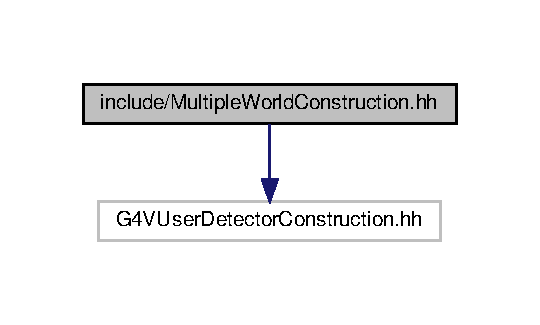
\includegraphics[width=259pt]{MultipleWorldConstruction_8hh__incl}
\end{center}
\end{figure}
This graph shows which files directly or indirectly include this file\+:
\nopagebreak
\begin{figure}[H]
\begin{center}
\leavevmode
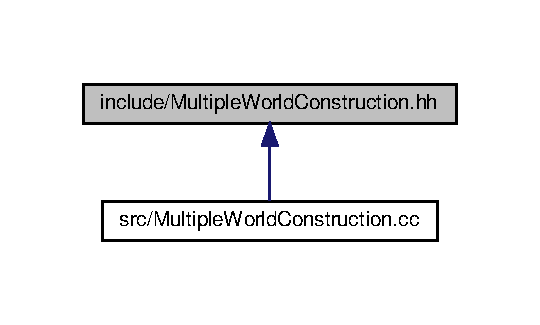
\includegraphics[width=259pt]{MultipleWorldConstruction_8hh__dep__incl}
\end{center}
\end{figure}
\subsection*{Classes}
\begin{DoxyCompactItemize}
\item 
class \hyperlink{classMultipleWorldConstruction}{Multiple\+World\+Construction}
\end{DoxyCompactItemize}


\subsection{Detailed Description}
multiple world construction header file, when used allows us to choose the world based on the input that we receive from the get\+Input function in main, but by default we use a G\+TK window instead. 

\begin{DoxyAuthor}{Author}
Oisin O\textquotesingle{}Connell
\end{DoxyAuthor}
\begin{DoxyDate}{Date}
7/20/20 
\end{DoxyDate}

\hypertarget{NeutronActionInitialization_8hh}{}\section{include/\+Neutron\+Action\+Initialization.hh File Reference}
\label{NeutronActionInitialization_8hh}\index{include/\+Neutron\+Action\+Initialization.\+hh@{include/\+Neutron\+Action\+Initialization.\+hh}}


neutron action initialization header file, where we initialize user actions such as defining the behavior for events and runs. Currently we are only defining user actions for the primary generator action and the run action.  


{\ttfamily \#include \char`\"{}G4\+V\+User\+Action\+Initialization.\+hh\char`\"{}}\newline
Include dependency graph for Neutron\+Action\+Initialization.\+hh\+:
\nopagebreak
\begin{figure}[H]
\begin{center}
\leavevmode
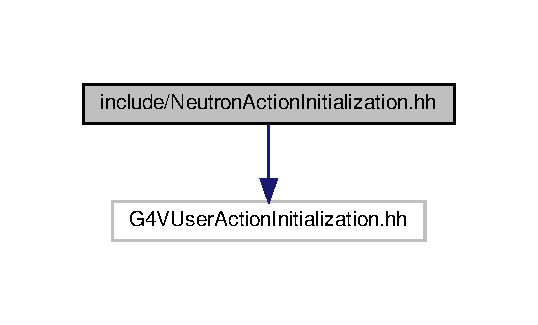
\includegraphics[width=258pt]{NeutronActionInitialization_8hh__incl}
\end{center}
\end{figure}
This graph shows which files directly or indirectly include this file\+:
\nopagebreak
\begin{figure}[H]
\begin{center}
\leavevmode
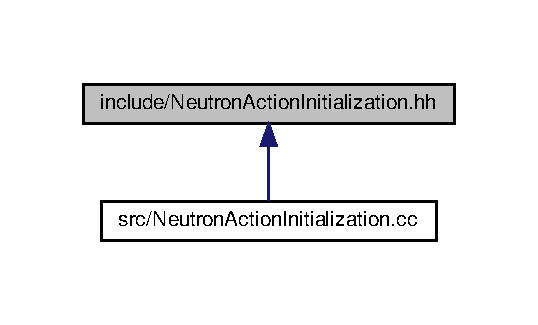
\includegraphics[width=258pt]{NeutronActionInitialization_8hh__dep__incl}
\end{center}
\end{figure}
\subsection*{Classes}
\begin{DoxyCompactItemize}
\item 
class \hyperlink{classNeutronActionInitialization}{Neutron\+Action\+Initialization}
\end{DoxyCompactItemize}


\subsection{Detailed Description}
neutron action initialization header file, where we initialize user actions such as defining the behavior for events and runs. Currently we are only defining user actions for the primary generator action and the run action. 

\begin{DoxyAuthor}{Author}
Oisin O\textquotesingle{}Connell
\end{DoxyAuthor}
\begin{DoxyDate}{Date}
7/20/20 
\end{DoxyDate}

\hypertarget{NeutronPrimaryGeneratorAction_8hh}{}\section{include/\+Neutron\+Primary\+Generator\+Action.hh File Reference}
\label{NeutronPrimaryGeneratorAction_8hh}\index{include/\+Neutron\+Primary\+Generator\+Action.\+hh@{include/\+Neutron\+Primary\+Generator\+Action.\+hh}}


primary generator action, where we create our thermal neutrons. We pass an instance of this derived class to the run manager in our derived class, \hyperlink{classNeutronActionInitialization}{Neutron\+Action\+Initialization}.  


{\ttfamily \#include \char`\"{}G4\+V\+User\+Primary\+Generator\+Action.\+hh\char`\"{}}\newline
{\ttfamily \#include \char`\"{}G4\+Particle\+Gun.\+hh\char`\"{}}\newline
Include dependency graph for Neutron\+Primary\+Generator\+Action.\+hh\+:
\nopagebreak
\begin{figure}[H]
\begin{center}
\leavevmode
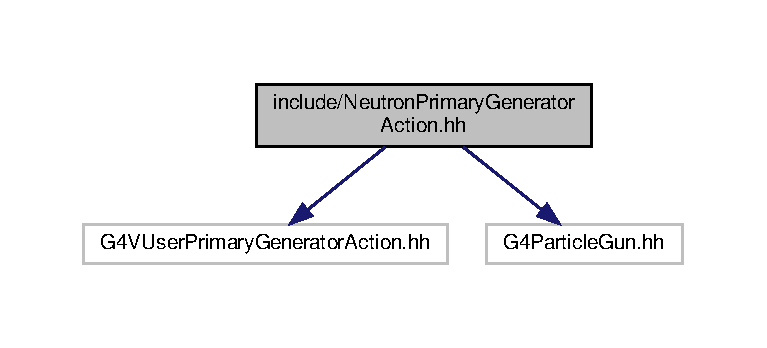
\includegraphics[width=350pt]{NeutronPrimaryGeneratorAction_8hh__incl}
\end{center}
\end{figure}
This graph shows which files directly or indirectly include this file\+:
\nopagebreak
\begin{figure}[H]
\begin{center}
\leavevmode
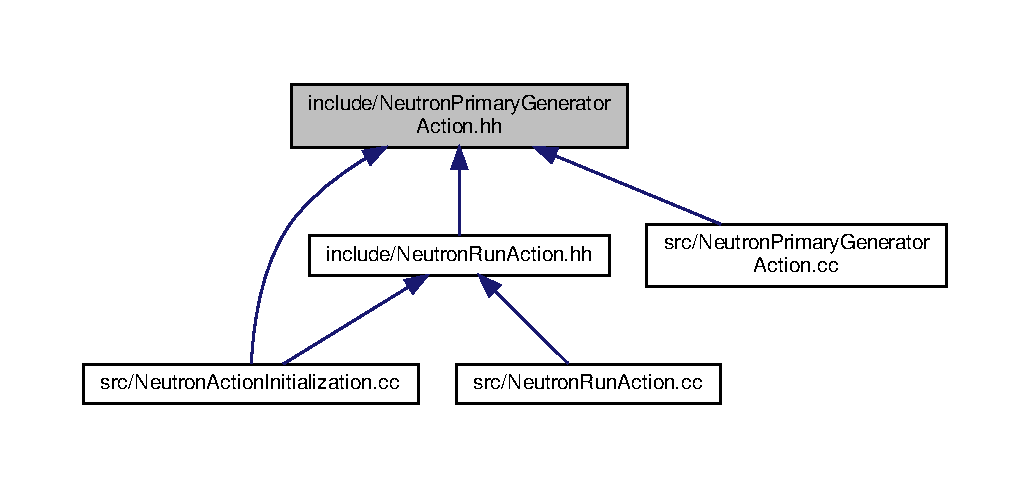
\includegraphics[width=350pt]{NeutronPrimaryGeneratorAction_8hh__dep__incl}
\end{center}
\end{figure}
\subsection*{Classes}
\begin{DoxyCompactItemize}
\item 
class \hyperlink{classNeutronPrimaryGeneratorAction}{Neutron\+Primary\+Generator\+Action}
\end{DoxyCompactItemize}


\subsection{Detailed Description}
primary generator action, where we create our thermal neutrons. We pass an instance of this derived class to the run manager in our derived class, \hyperlink{classNeutronActionInitialization}{Neutron\+Action\+Initialization}. 

\begin{DoxyAuthor}{Author}
Oisin O\textquotesingle{}Connell
\end{DoxyAuthor}
\begin{DoxyDate}{Date}
7/20/20 
\end{DoxyDate}

\hypertarget{NeutronRunAction_8hh}{}\section{include/\+Neutron\+Run\+Action.hh File Reference}
\label{NeutronRunAction_8hh}\index{include/\+Neutron\+Run\+Action.\+hh@{include/\+Neutron\+Run\+Action.\+hh}}


Run user action header file, allows us to define what should occur before and after a run. Currently being used to open and close the histogram if the user turns it on.  


{\ttfamily \#include \char`\"{}G4\+User\+Run\+Action.\+hh\char`\"{}}\newline
{\ttfamily \#include \char`\"{}Neutron\+Primary\+Generator\+Action.\+hh\char`\"{}}\newline
{\ttfamily \#include \char`\"{}G4\+Run.\+hh\char`\"{}}\newline
Include dependency graph for Neutron\+Run\+Action.\+hh\+:
\nopagebreak
\begin{figure}[H]
\begin{center}
\leavevmode
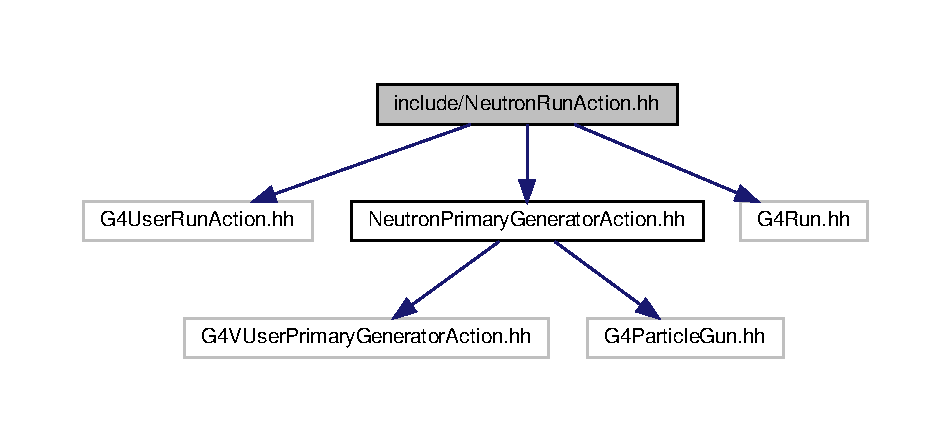
\includegraphics[width=350pt]{NeutronRunAction_8hh__incl}
\end{center}
\end{figure}
This graph shows which files directly or indirectly include this file\+:
\nopagebreak
\begin{figure}[H]
\begin{center}
\leavevmode
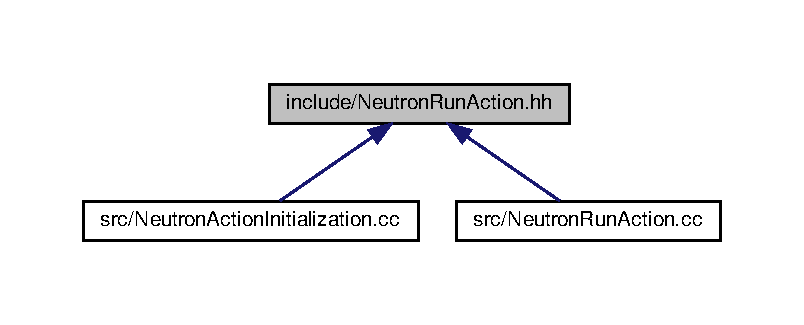
\includegraphics[width=350pt]{NeutronRunAction_8hh__dep__incl}
\end{center}
\end{figure}
\subsection*{Classes}
\begin{DoxyCompactItemize}
\item 
class \hyperlink{classNeutronRunAction}{Neutron\+Run\+Action}
\end{DoxyCompactItemize}


\subsection{Detailed Description}
Run user action header file, allows us to define what should occur before and after a run. Currently being used to open and close the histogram if the user turns it on. 

\begin{DoxyAuthor}{Author}
Oisin O\textquotesingle{}Connell 
\end{DoxyAuthor}
\begin{DoxyDate}{Date}
7/29/2020 
\end{DoxyDate}

\hypertarget{3HeDetectorConstruction_8cc}{}\section{src/3\+He\+Detector\+Construction.cc File Reference}
\label{3HeDetectorConstruction_8cc}\index{src/3\+He\+Detector\+Construction.\+cc@{src/3\+He\+Detector\+Construction.\+cc}}


helium-\/3 detector construction file. Air envelope with 3\+He container.  


{\ttfamily \#include \char`\"{}3\+He\+Detector\+Construction.\+hh\char`\"{}}\newline
{\ttfamily \#include \char`\"{}Counter\+S\+D.\+hh\char`\"{}}\newline
{\ttfamily \#include \char`\"{}G4\+S\+D\+Manager.\+hh\char`\"{}}\newline
{\ttfamily \#include \char`\"{}G4\+Run\+Manager.\+hh\char`\"{}}\newline
{\ttfamily \#include \char`\"{}G4\+Nist\+Manager.\+hh\char`\"{}}\newline
{\ttfamily \#include \char`\"{}G4\+Box.\+hh\char`\"{}}\newline
{\ttfamily \#include \char`\"{}G4\+P\+V\+Placement.\+hh\char`\"{}}\newline
{\ttfamily \#include \char`\"{}G4\+Logical\+Volume.\+hh\char`\"{}}\newline
{\ttfamily \#include \char`\"{}G4\+System\+Of\+Units.\+hh\char`\"{}}\newline
Include dependency graph for 3\+He\+Detector\+Construction.cc\+:
\nopagebreak
\begin{figure}[H]
\begin{center}
\leavevmode
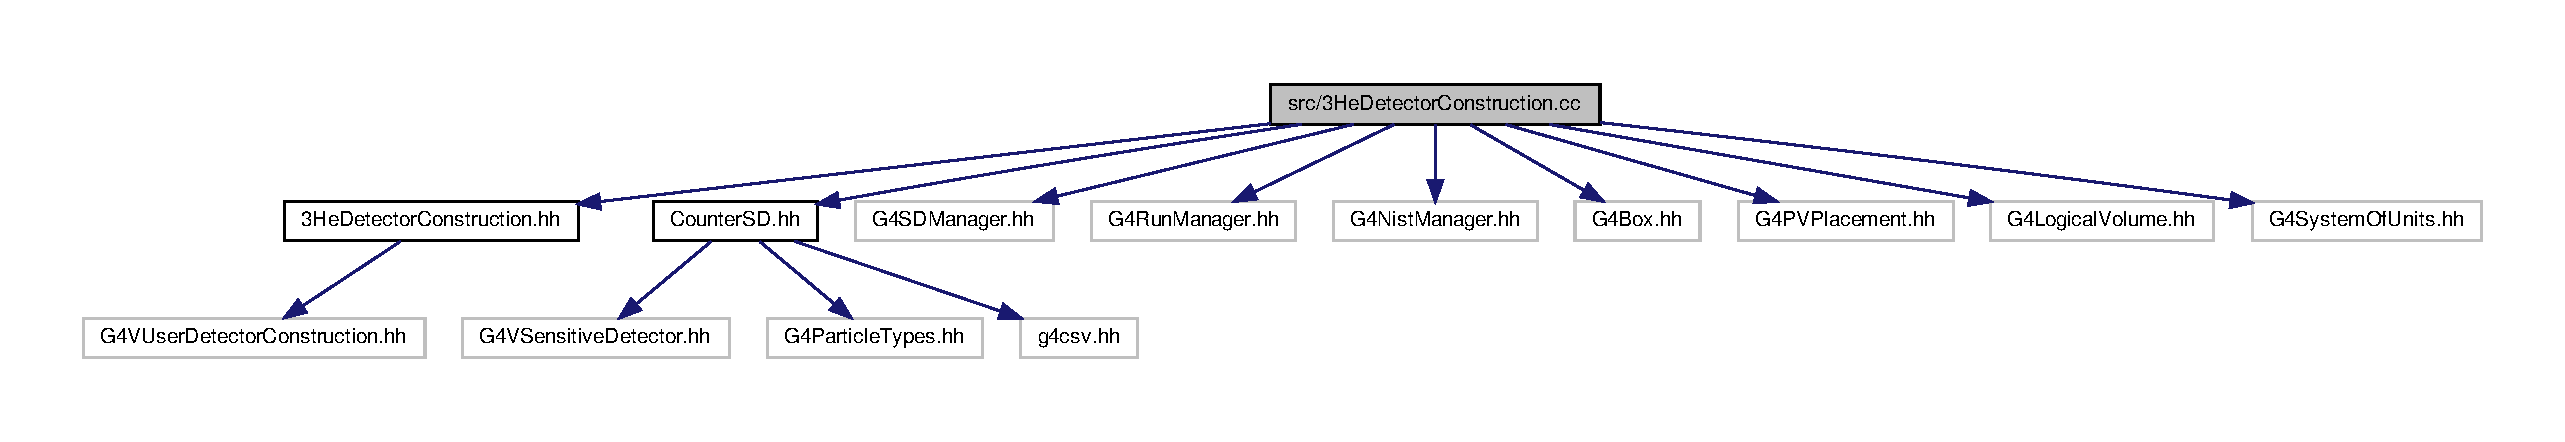
\includegraphics[width=350pt]{3HeDetectorConstruction_8cc__incl}
\end{center}
\end{figure}


\subsection{Detailed Description}
helium-\/3 detector construction file. Air envelope with 3\+He container. 

\begin{DoxyAuthor}{Author}
Oisin O\textquotesingle{}Connell 
\end{DoxyAuthor}
\begin{DoxyDate}{Date}
7/28/2020 
\end{DoxyDate}

\hypertarget{3HeWorldConstruction_8cc}{}\section{src/3\+He\+World\+Construction.cc File Reference}
\label{3HeWorldConstruction_8cc}\index{src/3\+He\+World\+Construction.\+cc@{src/3\+He\+World\+Construction.\+cc}}


helium-\/3 world envelope construction file.  


{\ttfamily \#include \char`\"{}3\+He\+World\+Construction.\+hh\char`\"{}}\newline
{\ttfamily \#include \char`\"{}G4\+Run\+Manager.\+hh\char`\"{}}\newline
{\ttfamily \#include \char`\"{}G4\+Nist\+Manager.\+hh\char`\"{}}\newline
{\ttfamily \#include \char`\"{}G4\+Box.\+hh\char`\"{}}\newline
{\ttfamily \#include \char`\"{}G4\+P\+V\+Placement.\+hh\char`\"{}}\newline
{\ttfamily \#include \char`\"{}G4\+Logical\+Volume.\+hh\char`\"{}}\newline
{\ttfamily \#include \char`\"{}G4\+System\+Of\+Units.\+hh\char`\"{}}\newline
Include dependency graph for 3\+He\+World\+Construction.cc\+:
\nopagebreak
\begin{figure}[H]
\begin{center}
\leavevmode
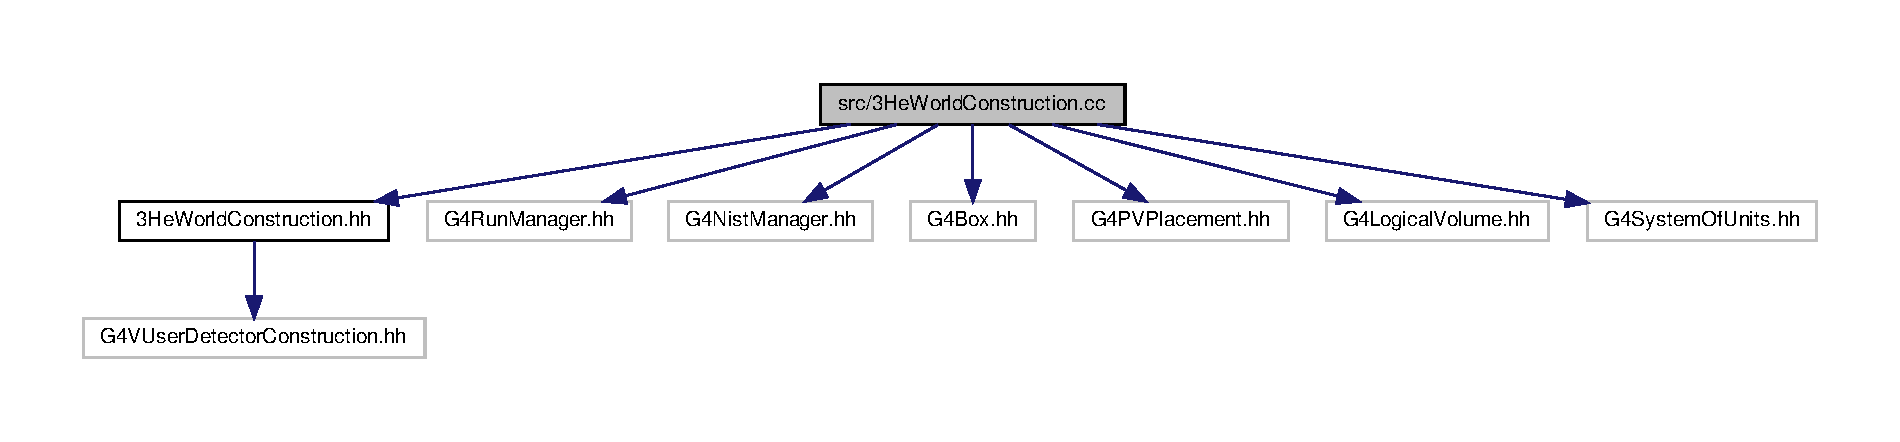
\includegraphics[width=350pt]{3HeWorldConstruction_8cc__incl}
\end{center}
\end{figure}


\subsection{Detailed Description}
helium-\/3 world envelope construction file. 

\begin{DoxyAuthor}{Author}
Oisin O\textquotesingle{}Connell 
\end{DoxyAuthor}
\begin{DoxyDate}{Date}
7/28/2020 
\end{DoxyDate}

\hypertarget{4HeDetectorConstruction_8cc}{}\section{src/4\+He\+Detector\+Construction.cc File Reference}
\label{4HeDetectorConstruction_8cc}\index{src/4\+He\+Detector\+Construction.\+cc@{src/4\+He\+Detector\+Construction.\+cc}}


helium-\/4 container in an air world envelope detector construction file  


{\ttfamily \#include \char`\"{}4\+He\+Detector\+Construction.\+hh\char`\"{}}\newline
{\ttfamily \#include \char`\"{}G4\+Run\+Manager.\+hh\char`\"{}}\newline
{\ttfamily \#include \char`\"{}G4\+Nist\+Manager.\+hh\char`\"{}}\newline
{\ttfamily \#include \char`\"{}G4\+Box.\+hh\char`\"{}}\newline
{\ttfamily \#include \char`\"{}G4\+P\+V\+Placement.\+hh\char`\"{}}\newline
{\ttfamily \#include \char`\"{}G4\+Logical\+Volume.\+hh\char`\"{}}\newline
{\ttfamily \#include \char`\"{}G4\+System\+Of\+Units.\+hh\char`\"{}}\newline
Include dependency graph for 4\+He\+Detector\+Construction.cc\+:
\nopagebreak
\begin{figure}[H]
\begin{center}
\leavevmode
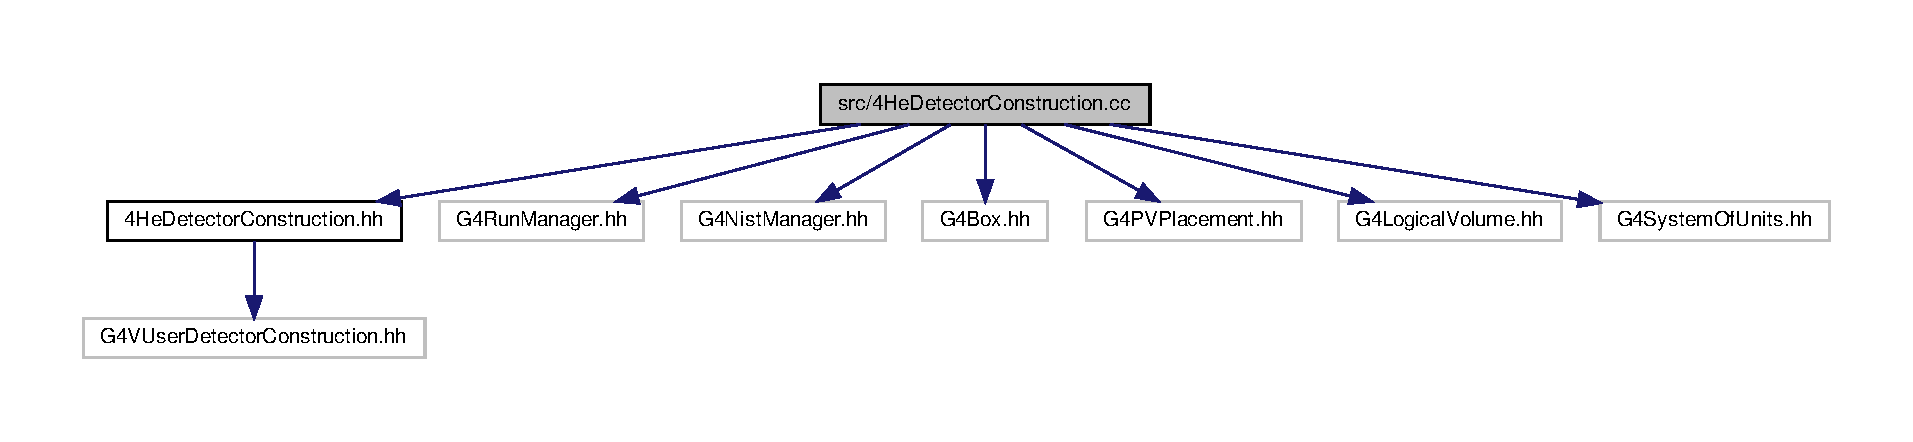
\includegraphics[width=350pt]{4HeDetectorConstruction_8cc__incl}
\end{center}
\end{figure}


\subsection{Detailed Description}
helium-\/4 container in an air world envelope detector construction file 

\begin{DoxyAuthor}{Author}
Oisin O\textquotesingle{}Connell 
\end{DoxyAuthor}
\begin{DoxyDate}{Date}
7/28/2020 
\end{DoxyDate}

\hypertarget{BF3DetectorConstruction_8cc}{}\section{src/\+B\+F3\+Detector\+Construction.cc File Reference}
\label{BF3DetectorConstruction_8cc}\index{src/\+B\+F3\+Detector\+Construction.\+cc@{src/\+B\+F3\+Detector\+Construction.\+cc}}


boron trifluoride container in a modifiable world envelope detector construction file  


{\ttfamily \#include \char`\"{}B\+F3\+Detector\+Construction.\+hh\char`\"{}}\newline
{\ttfamily \#include \char`\"{}Counter\+S\+D.\+hh\char`\"{}}\newline
{\ttfamily \#include \char`\"{}G\+T\+K\+Input.\+hh\char`\"{}}\newline
{\ttfamily \#include \char`\"{}G4\+S\+D\+Manager.\+hh\char`\"{}}\newline
{\ttfamily \#include \char`\"{}G4\+Run\+Manager.\+hh\char`\"{}}\newline
{\ttfamily \#include \char`\"{}G4\+Nist\+Manager.\+hh\char`\"{}}\newline
{\ttfamily \#include \char`\"{}G4\+Box.\+hh\char`\"{}}\newline
{\ttfamily \#include \char`\"{}G4\+P\+V\+Placement.\+hh\char`\"{}}\newline
{\ttfamily \#include \char`\"{}G4\+Logical\+Volume.\+hh\char`\"{}}\newline
{\ttfamily \#include \char`\"{}G4\+System\+Of\+Units.\+hh\char`\"{}}\newline
Include dependency graph for B\+F3\+Detector\+Construction.\+cc\+:
\nopagebreak
\begin{figure}[H]
\begin{center}
\leavevmode
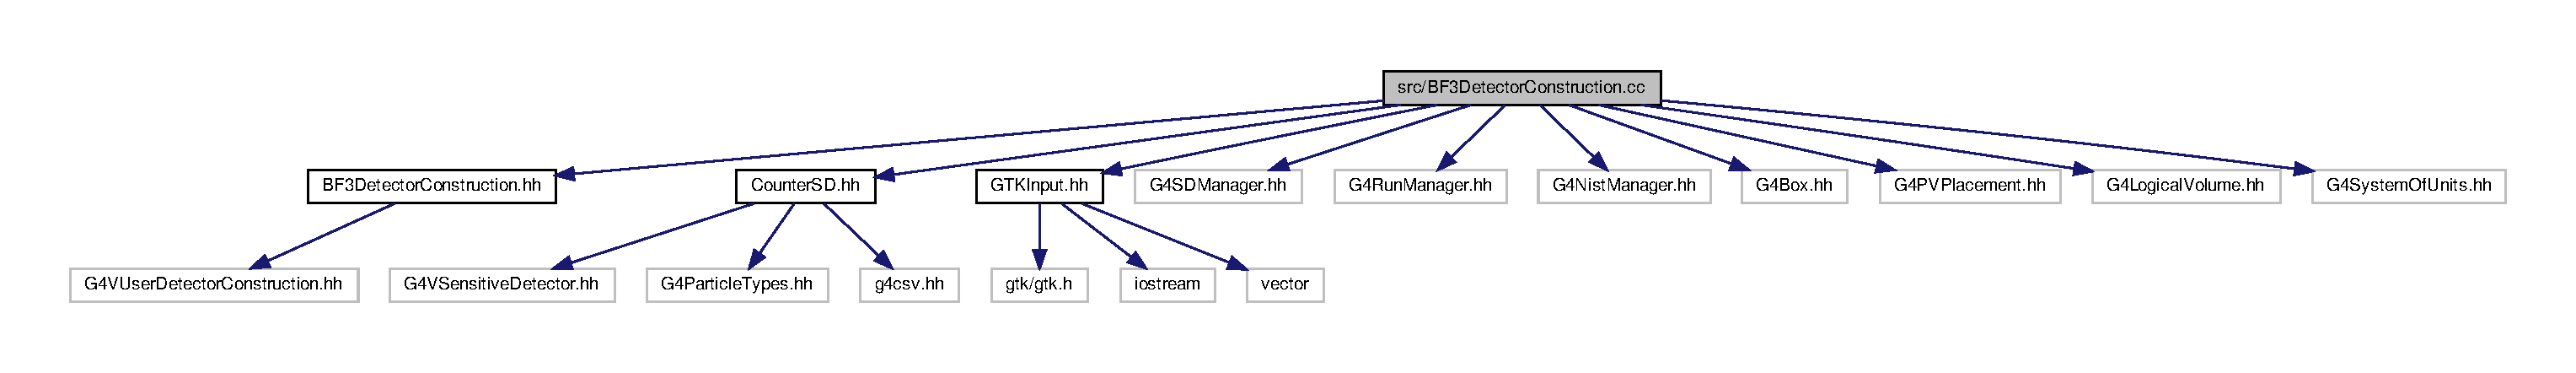
\includegraphics[width=350pt]{BF3DetectorConstruction_8cc__incl}
\end{center}
\end{figure}


\subsection{Detailed Description}
boron trifluoride container in a modifiable world envelope detector construction file 

\begin{DoxyAuthor}{Author}
Oisin O\textquotesingle{}Connell 
\end{DoxyAuthor}
\begin{DoxyDate}{Date}
7/28/2020 
\end{DoxyDate}

\hypertarget{CounterSD_8cc}{}\section{src/\+Counter\+SD.cc File Reference}
\label{CounterSD_8cc}\index{src/\+Counter\+S\+D.\+cc@{src/\+Counter\+S\+D.\+cc}}


sensitive detector definition file. We attach a sensitive detector to a logical volume in order to obtain energy deposition and other statistics for the volume.  


{\ttfamily \#include \char`\"{}Counter\+S\+D.\+hh\char`\"{}}\newline
{\ttfamily \#include \char`\"{}G\+T\+K\+Input.\+hh\char`\"{}}\newline
Include dependency graph for Counter\+S\+D.\+cc\+:
\nopagebreak
\begin{figure}[H]
\begin{center}
\leavevmode
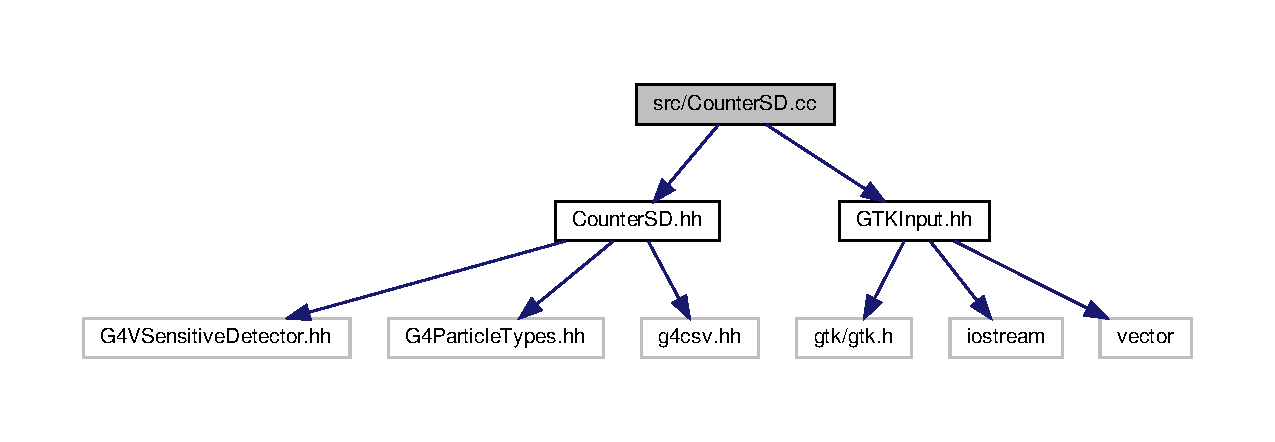
\includegraphics[width=350pt]{CounterSD_8cc__incl}
\end{center}
\end{figure}


\subsection{Detailed Description}
sensitive detector definition file. We attach a sensitive detector to a logical volume in order to obtain energy deposition and other statistics for the volume. 

\begin{DoxyAuthor}{Author}
Oisin O\textquotesingle{}Connell 
\end{DoxyAuthor}
\begin{DoxyDate}{Date}
7/28/2020 
\end{DoxyDate}

\hypertarget{GTKInput_8cc}{}\section{src/\+G\+T\+K\+Input.cc File Reference}
\label{GTKInput_8cc}\index{src/\+G\+T\+K\+Input.\+cc@{src/\+G\+T\+K\+Input.\+cc}}


G\+TK input file, allows user to input the material for the neutrons to propagate through and collects the user input in a struct that is used by the detector construction and the primary generator action to create a customized simulation.  


{\ttfamily \#include \char`\"{}G\+T\+K\+Input.\+hh\char`\"{}}\newline
Include dependency graph for G\+T\+K\+Input.\+cc\+:
\nopagebreak
\begin{figure}[H]
\begin{center}
\leavevmode
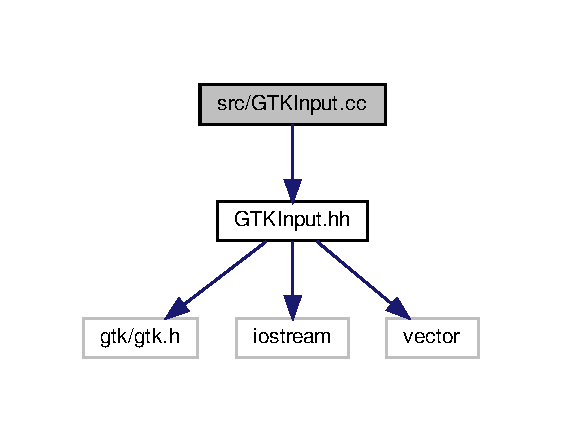
\includegraphics[width=270pt]{GTKInput_8cc__incl}
\end{center}
\end{figure}
\subsection*{Functions}
\begin{DoxyCompactItemize}
\item 
void \hyperlink{GTKInput_8cc_a3ab41ac6b7453a202f75619a5e8b16c3}{neutron\+\_\+energy\+\_\+insert\+\_\+event} (Gtk\+Editable $\ast$neutron\+\_\+energy, const gchar $\ast$text, gint length, gint $\ast$pos)
\begin{DoxyCompactList}\small\item\em prevents the entry of any non-\/numeric characters for the neutron energy \end{DoxyCompactList}\item 
void \hyperlink{GTKInput_8cc_a6d57308d4895545586446c43d2e58b25}{num\+\_\+events\+\_\+insert\+\_\+event} (Gtk\+Editable $\ast$events, const gchar $\ast$text, gint length, gint $\ast$pos)
\begin{DoxyCompactList}\small\item\em prevents the entry of any non-\/numeric characters for the number of events \end{DoxyCompactList}\item 
void \hyperlink{GTKInput_8cc_ab169f301782458153e7309e96de986c2}{submit\+\_\+clicked} (Gtk\+Widget $\ast$button, struct \hyperlink{structGTKBoxesContainer}{G\+T\+K\+Boxes\+Container} $\ast$multi\+\_\+arg)
\begin{DoxyCompactList}\small\item\em passes the inputted args to our global struct so that the simulation can use them. \end{DoxyCompactList}\item 
\mbox{\Hypertarget{GTKInput_8cc_a19f5912b30e5d38df0a3c0bfa9b794f2}\label{GTKInput_8cc_a19f5912b30e5d38df0a3c0bfa9b794f2}} 
void {\bfseries create\+\_\+data\+\_\+entry\+\_\+window} ()
\item 
\mbox{\Hypertarget{GTKInput_8cc_a554b759199ed3e9b24f109ade7af4178}\label{GTKInput_8cc_a554b759199ed3e9b24f109ade7af4178}} 
void {\bfseries create\+\_\+result\+\_\+labels} (Gtk\+Widget $\ast$outer\+\_\+box, Gtk\+Widget $\ast$result\+\_\+box)
\end{DoxyCompactItemize}
\subsection*{Variables}
\begin{DoxyCompactItemize}
\item 
\mbox{\Hypertarget{GTKInput_8cc_aefb2ae95fdd6ed4de4ff76a886180f24}\label{GTKInput_8cc_aefb2ae95fdd6ed4de4ff76a886180f24}} 
std\+::vector$<$ std\+::string $>$ {\bfseries detector\+\_\+materials}
\item 
struct \hyperlink{structGTKBoxesContainer}{G\+T\+K\+Boxes\+Container} $\ast$ {\bfseries results}
\item 
\hyperlink{classInputValues}{Input\+Values} $\ast$ {\bfseries input\+\_\+values}
\item 
\hyperlink{classOutputValues}{Output\+Values} $\ast$ {\bfseries output\+\_\+values}
\end{DoxyCompactItemize}


\subsection{Detailed Description}
G\+TK input file, allows user to input the material for the neutrons to propagate through and collects the user input in a struct that is used by the detector construction and the primary generator action to create a customized simulation. 

\begin{DoxyAuthor}{Author}
Oisin O\textquotesingle{}Connell 
\end{DoxyAuthor}
\begin{DoxyDate}{Date}
7/29/2020 
\end{DoxyDate}


\subsection{Function Documentation}
\mbox{\Hypertarget{GTKInput_8cc_a3ab41ac6b7453a202f75619a5e8b16c3}\label{GTKInput_8cc_a3ab41ac6b7453a202f75619a5e8b16c3}} 
\index{G\+T\+K\+Input.\+cc@{G\+T\+K\+Input.\+cc}!neutron\+\_\+energy\+\_\+insert\+\_\+event@{neutron\+\_\+energy\+\_\+insert\+\_\+event}}
\index{neutron\+\_\+energy\+\_\+insert\+\_\+event@{neutron\+\_\+energy\+\_\+insert\+\_\+event}!G\+T\+K\+Input.\+cc@{G\+T\+K\+Input.\+cc}}
\subsubsection{\texorpdfstring{neutron\+\_\+energy\+\_\+insert\+\_\+event()}{neutron\_energy\_insert\_event()}}
{\footnotesize\ttfamily void neutron\+\_\+energy\+\_\+insert\+\_\+event (\begin{DoxyParamCaption}\item[{Gtk\+Editable $\ast$}]{neutron\+\_\+energy,  }\item[{const gchar $\ast$}]{text,  }\item[{gint}]{length,  }\item[{gint $\ast$}]{pos }\end{DoxyParamCaption})}



prevents the entry of any non-\/numeric characters for the neutron energy 


\begin{DoxyParams}{Parameters}
{\em neutron\+\_\+energy} & the text box \\
\hline
{\em text} & the text that was added to the text box \\
\hline
{\em length} & the length of the added text \\
\hline
{\em pos} & the length of the added text \\
\hline
\end{DoxyParams}
\mbox{\Hypertarget{GTKInput_8cc_a6d57308d4895545586446c43d2e58b25}\label{GTKInput_8cc_a6d57308d4895545586446c43d2e58b25}} 
\index{G\+T\+K\+Input.\+cc@{G\+T\+K\+Input.\+cc}!num\+\_\+events\+\_\+insert\+\_\+event@{num\+\_\+events\+\_\+insert\+\_\+event}}
\index{num\+\_\+events\+\_\+insert\+\_\+event@{num\+\_\+events\+\_\+insert\+\_\+event}!G\+T\+K\+Input.\+cc@{G\+T\+K\+Input.\+cc}}
\subsubsection{\texorpdfstring{num\+\_\+events\+\_\+insert\+\_\+event()}{num\_events\_insert\_event()}}
{\footnotesize\ttfamily void num\+\_\+events\+\_\+insert\+\_\+event (\begin{DoxyParamCaption}\item[{Gtk\+Editable $\ast$}]{events,  }\item[{const gchar $\ast$}]{text,  }\item[{gint}]{length,  }\item[{gint $\ast$}]{pos }\end{DoxyParamCaption})}



prevents the entry of any non-\/numeric characters for the number of events 


\begin{DoxyParams}{Parameters}
{\em events} & the text box \\
\hline
{\em text} & the text that was added to the text box \\
\hline
{\em length} & the length of the added text \\
\hline
{\em pos} & the length of the added text \\
\hline
\end{DoxyParams}
\mbox{\Hypertarget{GTKInput_8cc_ab169f301782458153e7309e96de986c2}\label{GTKInput_8cc_ab169f301782458153e7309e96de986c2}} 
\index{G\+T\+K\+Input.\+cc@{G\+T\+K\+Input.\+cc}!submit\+\_\+clicked@{submit\+\_\+clicked}}
\index{submit\+\_\+clicked@{submit\+\_\+clicked}!G\+T\+K\+Input.\+cc@{G\+T\+K\+Input.\+cc}}
\subsubsection{\texorpdfstring{submit\+\_\+clicked()}{submit\_clicked()}}
{\footnotesize\ttfamily void submit\+\_\+clicked (\begin{DoxyParamCaption}\item[{Gtk\+Widget $\ast$}]{button,  }\item[{struct \hyperlink{structGTKBoxesContainer}{G\+T\+K\+Boxes\+Container} $\ast$}]{multi\+\_\+arg }\end{DoxyParamCaption})}



passes the inputted args to our global struct so that the simulation can use them. 


\begin{DoxyParams}{Parameters}
{\em button} & the input button \\
\hline
{\em multi\+\_\+arg} & the struct containing the entered values \\
\hline
\end{DoxyParams}


\subsection{Variable Documentation}
\mbox{\Hypertarget{GTKInput_8cc_a69055fa214854d483b97260a00cbfa60}\label{GTKInput_8cc_a69055fa214854d483b97260a00cbfa60}} 
\index{G\+T\+K\+Input.\+cc@{G\+T\+K\+Input.\+cc}!input\+\_\+values@{input\+\_\+values}}
\index{input\+\_\+values@{input\+\_\+values}!G\+T\+K\+Input.\+cc@{G\+T\+K\+Input.\+cc}}
\subsubsection{\texorpdfstring{input\+\_\+values}{input\_values}}
{\footnotesize\ttfamily \hyperlink{classInputValues}{Input\+Values}$\ast$ input\+\_\+values}

{\bfseries Initial value\+:}
\begin{DoxyCode}
=
    (\hyperlink{classInputValues}{InputValues}*)malloc(\textcolor{keyword}{sizeof}(\hyperlink{classInputValues}{InputValues}))
\end{DoxyCode}
\mbox{\Hypertarget{GTKInput_8cc_af802813aa13c8a2d9a86f12dc49d5c92}\label{GTKInput_8cc_af802813aa13c8a2d9a86f12dc49d5c92}} 
\index{G\+T\+K\+Input.\+cc@{G\+T\+K\+Input.\+cc}!output\+\_\+values@{output\+\_\+values}}
\index{output\+\_\+values@{output\+\_\+values}!G\+T\+K\+Input.\+cc@{G\+T\+K\+Input.\+cc}}
\subsubsection{\texorpdfstring{output\+\_\+values}{output\_values}}
{\footnotesize\ttfamily \hyperlink{classOutputValues}{Output\+Values}$\ast$ output\+\_\+values}

{\bfseries Initial value\+:}
\begin{DoxyCode}
=
    (\hyperlink{classOutputValues}{OutputValues}*)malloc(\textcolor{keyword}{sizeof}(\hyperlink{classOutputValues}{OutputValues}))
\end{DoxyCode}
\mbox{\Hypertarget{GTKInput_8cc_a9af02616a624ef7c34dee19b71e0bf32}\label{GTKInput_8cc_a9af02616a624ef7c34dee19b71e0bf32}} 
\index{G\+T\+K\+Input.\+cc@{G\+T\+K\+Input.\+cc}!results@{results}}
\index{results@{results}!G\+T\+K\+Input.\+cc@{G\+T\+K\+Input.\+cc}}
\subsubsection{\texorpdfstring{results}{results}}
{\footnotesize\ttfamily struct \hyperlink{structGTKBoxesContainer}{G\+T\+K\+Boxes\+Container}$\ast$ results}

{\bfseries Initial value\+:}
\begin{DoxyCode}
=
    (\hyperlink{structGTKBoxesContainer}{GTKBoxesContainer}*)malloc(\textcolor{keyword}{sizeof}(\hyperlink{structGTKBoxesContainer}{GTKBoxesContainer}))
\end{DoxyCode}

\hypertarget{GTKOutput_8cc}{}\section{src/\+G\+T\+K\+Output.cc File Reference}
\label{GTKOutput_8cc}\index{src/\+G\+T\+K\+Output.\+cc@{src/\+G\+T\+K\+Output.\+cc}}


G\+TK output file, collects the results from the \hyperlink{classOutputValues}{Output\+Values} struct that is forward declared in the G\+T\+K\+Input header file and displays them as the output.  


{\ttfamily \#include \char`\"{}G\+T\+K\+Input.\+hh\char`\"{}}\newline
{\ttfamily \#include \char`\"{}G\+T\+K\+Output.\+hh\char`\"{}}\newline
{\ttfamily \#include $<$sstream$>$}\newline
{\ttfamily \#include $<$iomanip$>$}\newline
Include dependency graph for G\+T\+K\+Output.\+cc\+:
\nopagebreak
\begin{figure}[H]
\begin{center}
\leavevmode
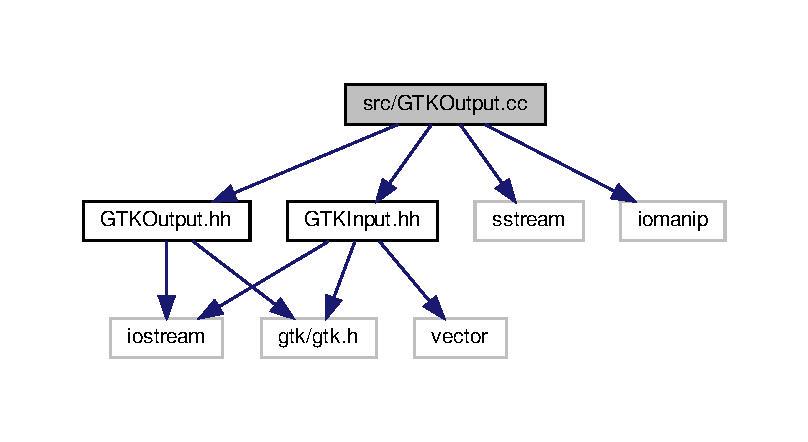
\includegraphics[width=350pt]{GTKOutput_8cc__incl}
\end{center}
\end{figure}
\subsection*{Functions}
\begin{DoxyCompactItemize}
\item 
\mbox{\Hypertarget{GTKOutput_8cc_a6391991aa8e57c5bdfae21fb4fd8f707}\label{GTKOutput_8cc_a6391991aa8e57c5bdfae21fb4fd8f707}} 
void \hyperlink{GTKOutput_8cc_a6391991aa8e57c5bdfae21fb4fd8f707}{create\+\_\+output\+\_\+window} ()
\begin{DoxyCompactList}\small\item\em creates the output window that contains the energy deposition and other statistics after a simulation has run. \end{DoxyCompactList}\item 
void \hyperlink{GTKOutput_8cc_acc11cbf62638ba1237401d4346d86a1c}{close\+\_\+clicked} (Gtk\+Widget $\ast$button, struct \hyperlink{structWinContainer}{Win\+Container} $\ast$wc)
\begin{DoxyCompactList}\small\item\em callback that closes the window when the close button is clicked \end{DoxyCompactList}\end{DoxyCompactItemize}


\subsection{Detailed Description}
G\+TK output file, collects the results from the \hyperlink{classOutputValues}{Output\+Values} struct that is forward declared in the G\+T\+K\+Input header file and displays them as the output. 

\begin{DoxyAuthor}{Author}
Oisin O\textquotesingle{}Connell 
\end{DoxyAuthor}
\begin{DoxyDate}{Date}
7/29/2020 
\end{DoxyDate}


\subsection{Function Documentation}
\mbox{\Hypertarget{GTKOutput_8cc_acc11cbf62638ba1237401d4346d86a1c}\label{GTKOutput_8cc_acc11cbf62638ba1237401d4346d86a1c}} 
\index{G\+T\+K\+Output.\+cc@{G\+T\+K\+Output.\+cc}!close\+\_\+clicked@{close\+\_\+clicked}}
\index{close\+\_\+clicked@{close\+\_\+clicked}!G\+T\+K\+Output.\+cc@{G\+T\+K\+Output.\+cc}}
\subsubsection{\texorpdfstring{close\+\_\+clicked()}{close\_clicked()}}
{\footnotesize\ttfamily void close\+\_\+clicked (\begin{DoxyParamCaption}\item[{Gtk\+Widget $\ast$}]{button,  }\item[{struct \hyperlink{structWinContainer}{Win\+Container} $\ast$}]{wc }\end{DoxyParamCaption})}



callback that closes the window when the close button is clicked 


\begin{DoxyParams}{Parameters}
{\em button} & the button widget \\
\hline
{\em wc} & a struct containing the window that displays the results \\
\hline
\end{DoxyParams}

\hypertarget{HistogramsAnalysisManager_8cc}{}\section{src/\+Histograms\+Analysis\+Manager.cc File Reference}
\label{HistogramsAnalysisManager_8cc}\index{src/\+Histograms\+Analysis\+Manager.\+cc@{src/\+Histograms\+Analysis\+Manager.\+cc}}


Analysis manager file, optionally allows us to place commands within our code that add to a histogram based on an event, a step, or something else.  


{\ttfamily \#include \char`\"{}Histograms\+Analysis\+Manager.\+hh\char`\"{}}\newline
{\ttfamily \#include \char`\"{}G4\+Units\+Table.\+hh\char`\"{}}\newline
Include dependency graph for Histograms\+Analysis\+Manager.\+cc\+:
\nopagebreak
\begin{figure}[H]
\begin{center}
\leavevmode
\includegraphics[width=344pt]{HistogramsAnalysisManager_8cc__incl}
\end{center}
\end{figure}


\subsection{Detailed Description}
Analysis manager file, optionally allows us to place commands within our code that add to a histogram based on an event, a step, or something else. 

\begin{DoxyAuthor}{Author}
Oisin O\textquotesingle{}Connell 
\end{DoxyAuthor}
\begin{DoxyDate}{Date}
7/29/2020 
\end{DoxyDate}

\hypertarget{MultipleWorldConstruction_8cc}{}\section{src/\+Multiple\+World\+Construction.cc File Reference}
\label{MultipleWorldConstruction_8cc}\index{src/\+Multiple\+World\+Construction.\+cc@{src/\+Multiple\+World\+Construction.\+cc}}


multiple world construction header file, when used allows us to choose the world based on the input that we receive from the get\+Input function in main, but by default we use a G\+TK window instead.  


{\ttfamily \#include \char`\"{}Multiple\+World\+Construction.\+hh\char`\"{}}\newline
{\ttfamily \#include \char`\"{}G4\+Run\+Manager.\+hh\char`\"{}}\newline
{\ttfamily \#include \char`\"{}G4\+Nist\+Manager.\+hh\char`\"{}}\newline
{\ttfamily \#include \char`\"{}G4\+Box.\+hh\char`\"{}}\newline
{\ttfamily \#include \char`\"{}G4\+P\+V\+Placement.\+hh\char`\"{}}\newline
{\ttfamily \#include \char`\"{}G4\+Logical\+Volume.\+hh\char`\"{}}\newline
{\ttfamily \#include \char`\"{}G4\+System\+Of\+Units.\+hh\char`\"{}}\newline
Include dependency graph for Multiple\+World\+Construction.\+cc\+:
\nopagebreak
\begin{figure}[H]
\begin{center}
\leavevmode
\includegraphics[width=350pt]{MultipleWorldConstruction_8cc__incl}
\end{center}
\end{figure}
\subsection*{Variables}
\begin{DoxyCompactItemize}
\item 
\mbox{\Hypertarget{MultipleWorldConstruction_8cc_a2949513d4205c97accdb512267b16078}\label{MultipleWorldConstruction_8cc_a2949513d4205c97accdb512267b16078}} 
int {\bfseries A\+I\+R\+\_\+\+S\+E\+L\+E\+C\+T\+ED}
\item 
\mbox{\Hypertarget{MultipleWorldConstruction_8cc_a93d9d1add1c17e2ae9723c89f77f047f}\label{MultipleWorldConstruction_8cc_a93d9d1add1c17e2ae9723c89f77f047f}} 
int {\bfseries S\+P\+A\+C\+E\+\_\+\+S\+E\+L\+E\+C\+T\+ED}
\item 
\mbox{\Hypertarget{MultipleWorldConstruction_8cc_af1d2cdb32af85fa8dcc407090d968c52}\label{MultipleWorldConstruction_8cc_af1d2cdb32af85fa8dcc407090d968c52}} 
int {\bfseries W\+A\+T\+E\+R\+\_\+\+S\+E\+L\+E\+C\+T\+ED}
\item 
\mbox{\Hypertarget{MultipleWorldConstruction_8cc_a74dc696d6118c25b84a895708dacf92a}\label{MultipleWorldConstruction_8cc_a74dc696d6118c25b84a895708dacf92a}} 
int {\bfseries A\+R\+G\+O\+N\+\_\+\+S\+E\+L\+E\+C\+T\+ED}
\item 
\mbox{\Hypertarget{MultipleWorldConstruction_8cc_a5791b97ab4cdc578a6e9f013484d87ac}\label{MultipleWorldConstruction_8cc_a5791b97ab4cdc578a6e9f013484d87ac}} 
int {\bfseries H\+E\+L\+I\+U\+M\+\_\+\+S\+E\+L\+E\+C\+T\+ED}
\end{DoxyCompactItemize}


\subsection{Detailed Description}
multiple world construction header file, when used allows us to choose the world based on the input that we receive from the get\+Input function in main, but by default we use a G\+TK window instead. 

\begin{DoxyAuthor}{Author}
Oisin O\textquotesingle{}Connell
\end{DoxyAuthor}
\begin{DoxyDate}{Date}
7/20/20 
\end{DoxyDate}

\hypertarget{NeutronActionInitialization_8cc}{}\section{src/\+Neutron\+Action\+Initialization.cc File Reference}
\label{NeutronActionInitialization_8cc}\index{src/\+Neutron\+Action\+Initialization.\+cc@{src/\+Neutron\+Action\+Initialization.\+cc}}


neutron action initialization header file, where we initialize user actions such as defining the behavior for events and runs. Currently we are only defining user actions for the primary generator action and the run action.  


{\ttfamily \#include \char`\"{}Neutron\+Action\+Initialization.\+hh\char`\"{}}\newline
{\ttfamily \#include \char`\"{}Neutron\+Primary\+Generator\+Action.\+hh\char`\"{}}\newline
{\ttfamily \#include \char`\"{}Neutron\+Run\+Action.\+hh\char`\"{}}\newline
Include dependency graph for Neutron\+Action\+Initialization.\+cc\+:
\nopagebreak
\begin{figure}[H]
\begin{center}
\leavevmode
\includegraphics[width=350pt]{NeutronActionInitialization_8cc__incl}
\end{center}
\end{figure}


\subsection{Detailed Description}
neutron action initialization header file, where we initialize user actions such as defining the behavior for events and runs. Currently we are only defining user actions for the primary generator action and the run action. 

\begin{DoxyAuthor}{Author}
Oisin O\textquotesingle{}Connell
\end{DoxyAuthor}
\begin{DoxyDate}{Date}
7/20/20 
\end{DoxyDate}

\hypertarget{NeutronPrimaryGeneratorAction_8cc}{}\section{src/\+Neutron\+Primary\+Generator\+Action.cc File Reference}
\label{NeutronPrimaryGeneratorAction_8cc}\index{src/\+Neutron\+Primary\+Generator\+Action.\+cc@{src/\+Neutron\+Primary\+Generator\+Action.\+cc}}


constructs the particle gun and initializes the particle generation when used as a user action in the \hyperlink{classNeutronActionInitialization}{Neutron\+Action\+Initialization} class  


{\ttfamily \#include \char`\"{}Neutron\+Primary\+Generator\+Action.\+hh\char`\"{}}\newline
{\ttfamily \#include \char`\"{}G\+T\+K\+Input.\+hh\char`\"{}}\newline
{\ttfamily \#include \char`\"{}G4\+System\+Of\+Units.\+hh\char`\"{}}\newline
{\ttfamily \#include \char`\"{}G4\+Particle\+Definition.\+hh\char`\"{}}\newline
{\ttfamily \#include \char`\"{}G4\+Particle\+Gun.\+hh\char`\"{}}\newline
{\ttfamily \#include \char`\"{}G4\+Particle\+Table.\+hh\char`\"{}}\newline
{\ttfamily \#include \char`\"{}Randomize.\+hh\char`\"{}}\newline
Include dependency graph for Neutron\+Primary\+Generator\+Action.\+cc\+:
\nopagebreak
\begin{figure}[H]
\begin{center}
\leavevmode
\includegraphics[width=350pt]{NeutronPrimaryGeneratorAction_8cc__incl}
\end{center}
\end{figure}


\subsection{Detailed Description}
constructs the particle gun and initializes the particle generation when used as a user action in the \hyperlink{classNeutronActionInitialization}{Neutron\+Action\+Initialization} class 

\begin{DoxyAuthor}{Author}
Oisin O\textquotesingle{}Connell
\end{DoxyAuthor}
\begin{DoxyDate}{Date}
7/20/20 
\end{DoxyDate}

\hypertarget{NeutronRunAction_8cc}{}\section{src/\+Neutron\+Run\+Action.cc File Reference}
\label{NeutronRunAction_8cc}\index{src/\+Neutron\+Run\+Action.\+cc@{src/\+Neutron\+Run\+Action.\+cc}}


Run user action file, allows us to define what should occur before and after a run. Currently being used to open and close the histogram if the user turns it on.  


{\ttfamily \#include \char`\"{}Neutron\+Run\+Action.\+hh\char`\"{}}\newline
{\ttfamily \#include \char`\"{}Histograms\+Analysis\+Manager.\+hh\char`\"{}}\newline
Include dependency graph for Neutron\+Run\+Action.\+cc\+:
\nopagebreak
\begin{figure}[H]
\begin{center}
\leavevmode
\includegraphics[width=350pt]{NeutronRunAction_8cc__incl}
\end{center}
\end{figure}


\subsection{Detailed Description}
Run user action file, allows us to define what should occur before and after a run. Currently being used to open and close the histogram if the user turns it on. 

\begin{DoxyAuthor}{Author}
Oisin O\textquotesingle{}Connell 
\end{DoxyAuthor}
\begin{DoxyDate}{Date}
7/29/2020 
\end{DoxyDate}

%--- End generated contents ---

% Index
\backmatter
\newpage
\phantomsection
\clearemptydoublepage
\addcontentsline{toc}{chapter}{Index}
\printindex

\end{document}
